% Options for packages loaded elsewhere
\PassOptionsToPackage{unicode}{hyperref}
\PassOptionsToPackage{hyphens}{url}
%
\documentclass[
]{article}
\usepackage{amsmath,amssymb}
\usepackage{iftex}
\ifPDFTeX
  \usepackage[T1]{fontenc}
  \usepackage[utf8]{inputenc}
  \usepackage{textcomp} % provide euro and other symbols
\else % if luatex or xetex
  \usepackage{unicode-math} % this also loads fontspec
  \defaultfontfeatures{Scale=MatchLowercase}
  \defaultfontfeatures[\rmfamily]{Ligatures=TeX,Scale=1}
\fi
\usepackage{lmodern}
\ifPDFTeX\else
  % xetex/luatex font selection
\fi
% Use upquote if available, for straight quotes in verbatim environments
\IfFileExists{upquote.sty}{\usepackage{upquote}}{}
\IfFileExists{microtype.sty}{% use microtype if available
  \usepackage[]{microtype}
  \UseMicrotypeSet[protrusion]{basicmath} % disable protrusion for tt fonts
}{}
\makeatletter
\@ifundefined{KOMAClassName}{% if non-KOMA class
  \IfFileExists{parskip.sty}{%
    \usepackage{parskip}
  }{% else
    \setlength{\parindent}{0pt}
    \setlength{\parskip}{6pt plus 2pt minus 1pt}}
}{% if KOMA class
  \KOMAoptions{parskip=half}}
\makeatother
\usepackage{xcolor}
\usepackage[margin=1in]{geometry}
\usepackage{color}
\usepackage{fancyvrb}
\newcommand{\VerbBar}{|}
\newcommand{\VERB}{\Verb[commandchars=\\\{\}]}
\DefineVerbatimEnvironment{Highlighting}{Verbatim}{commandchars=\\\{\}}
% Add ',fontsize=\small' for more characters per line
\usepackage{framed}
\definecolor{shadecolor}{RGB}{248,248,248}
\newenvironment{Shaded}{\begin{snugshade}}{\end{snugshade}}
\newcommand{\AlertTok}[1]{\textcolor[rgb]{0.94,0.16,0.16}{#1}}
\newcommand{\AnnotationTok}[1]{\textcolor[rgb]{0.56,0.35,0.01}{\textbf{\textit{#1}}}}
\newcommand{\AttributeTok}[1]{\textcolor[rgb]{0.13,0.29,0.53}{#1}}
\newcommand{\BaseNTok}[1]{\textcolor[rgb]{0.00,0.00,0.81}{#1}}
\newcommand{\BuiltInTok}[1]{#1}
\newcommand{\CharTok}[1]{\textcolor[rgb]{0.31,0.60,0.02}{#1}}
\newcommand{\CommentTok}[1]{\textcolor[rgb]{0.56,0.35,0.01}{\textit{#1}}}
\newcommand{\CommentVarTok}[1]{\textcolor[rgb]{0.56,0.35,0.01}{\textbf{\textit{#1}}}}
\newcommand{\ConstantTok}[1]{\textcolor[rgb]{0.56,0.35,0.01}{#1}}
\newcommand{\ControlFlowTok}[1]{\textcolor[rgb]{0.13,0.29,0.53}{\textbf{#1}}}
\newcommand{\DataTypeTok}[1]{\textcolor[rgb]{0.13,0.29,0.53}{#1}}
\newcommand{\DecValTok}[1]{\textcolor[rgb]{0.00,0.00,0.81}{#1}}
\newcommand{\DocumentationTok}[1]{\textcolor[rgb]{0.56,0.35,0.01}{\textbf{\textit{#1}}}}
\newcommand{\ErrorTok}[1]{\textcolor[rgb]{0.64,0.00,0.00}{\textbf{#1}}}
\newcommand{\ExtensionTok}[1]{#1}
\newcommand{\FloatTok}[1]{\textcolor[rgb]{0.00,0.00,0.81}{#1}}
\newcommand{\FunctionTok}[1]{\textcolor[rgb]{0.13,0.29,0.53}{\textbf{#1}}}
\newcommand{\ImportTok}[1]{#1}
\newcommand{\InformationTok}[1]{\textcolor[rgb]{0.56,0.35,0.01}{\textbf{\textit{#1}}}}
\newcommand{\KeywordTok}[1]{\textcolor[rgb]{0.13,0.29,0.53}{\textbf{#1}}}
\newcommand{\NormalTok}[1]{#1}
\newcommand{\OperatorTok}[1]{\textcolor[rgb]{0.81,0.36,0.00}{\textbf{#1}}}
\newcommand{\OtherTok}[1]{\textcolor[rgb]{0.56,0.35,0.01}{#1}}
\newcommand{\PreprocessorTok}[1]{\textcolor[rgb]{0.56,0.35,0.01}{\textit{#1}}}
\newcommand{\RegionMarkerTok}[1]{#1}
\newcommand{\SpecialCharTok}[1]{\textcolor[rgb]{0.81,0.36,0.00}{\textbf{#1}}}
\newcommand{\SpecialStringTok}[1]{\textcolor[rgb]{0.31,0.60,0.02}{#1}}
\newcommand{\StringTok}[1]{\textcolor[rgb]{0.31,0.60,0.02}{#1}}
\newcommand{\VariableTok}[1]{\textcolor[rgb]{0.00,0.00,0.00}{#1}}
\newcommand{\VerbatimStringTok}[1]{\textcolor[rgb]{0.31,0.60,0.02}{#1}}
\newcommand{\WarningTok}[1]{\textcolor[rgb]{0.56,0.35,0.01}{\textbf{\textit{#1}}}}
\usepackage{longtable,booktabs,array}
\usepackage{calc} % for calculating minipage widths
% Correct order of tables after \paragraph or \subparagraph
\usepackage{etoolbox}
\makeatletter
\patchcmd\longtable{\par}{\if@noskipsec\mbox{}\fi\par}{}{}
\makeatother
% Allow footnotes in longtable head/foot
\IfFileExists{footnotehyper.sty}{\usepackage{footnotehyper}}{\usepackage{footnote}}
\makesavenoteenv{longtable}
\usepackage{graphicx}
\makeatletter
\def\maxwidth{\ifdim\Gin@nat@width>\linewidth\linewidth\else\Gin@nat@width\fi}
\def\maxheight{\ifdim\Gin@nat@height>\textheight\textheight\else\Gin@nat@height\fi}
\makeatother
% Scale images if necessary, so that they will not overflow the page
% margins by default, and it is still possible to overwrite the defaults
% using explicit options in \includegraphics[width, height, ...]{}
\setkeys{Gin}{width=\maxwidth,height=\maxheight,keepaspectratio}
% Set default figure placement to htbp
\makeatletter
\def\fps@figure{htbp}
\makeatother
\setlength{\emergencystretch}{3em} % prevent overfull lines
\providecommand{\tightlist}{%
  \setlength{\itemsep}{0pt}\setlength{\parskip}{0pt}}
\setcounter{secnumdepth}{5}
\ifLuaTeX
  \usepackage{selnolig}  % disable illegal ligatures
\fi
\usepackage{bookmark}
\IfFileExists{xurl.sty}{\usepackage{xurl}}{} % add URL line breaks if available
\urlstyle{same}
\hypersetup{
  pdftitle={Statistical Learning Final Report},
  pdfauthor={Alberto Calabrese, Eleonora Mesaglio, Greta d'Amore Grelli},
  hidelinks,
  pdfcreator={LaTeX via pandoc}}

\title{Statistical Learning Final Report}
\author{Alberto Calabrese, Eleonora Mesaglio, Greta d'Amore Grelli}
\date{2024-06-14}

\begin{document}
\maketitle

{
\setcounter{tocdepth}{3}
\tableofcontents
}
\section{Introduction}\label{introduction}

In this project, we will conduct a thorough analysis of a dataset of our
choice, to gain a full understanding of our data, and we will then build
models that enable us to make accurate predictions. The dataset we chose
is called \emph{Starbucks Beverage Components} and contains information
about the ingredients of Starbucks' beverages.

We will go through several steps, including Data Cleaning, Exploratory
Data Analysis (EDA) and Regression Analysis. Indeed, first we will
prepare our data for analysis by handling missing values and ensuring
that our data is correctly formatted. Once our data is clean, we will
proceed to the EDA stage, where we will avail ourself of visual and
quantitative methods to understand the structure of our data and the
relationships between variables. Finally, we will perform Regression
Analysis to understand the relationship between our dependent and
independent variables. This will allow us to make predictions about our
data and understand the factors that influence our dependent variable,
\texttt{"Calories"}.

\section{Data}\label{data}

The dataset we will analyze in this project is \emph{Starbucks Beverage
Components} from Kaggle, that you can find at the following link:
\url{https://www.kaggle.com/datasets/henryshan/starbucks}.

This data provides a comprehensive guide to the nutritional content of
the beverages available on the Starbucks menu. We have a total of
\(242\) samples described by \(18\) variables. These attributes include
the name of the beverage, its categorization and preparation method, the
total caloric content and the constituents of the beverage.

\begin{Shaded}
\begin{Highlighting}[]
\NormalTok{data }\OtherTok{\textless{}{-}} \FunctionTok{read.csv}\NormalTok{(}\StringTok{"Data/starbucks.csv"}\NormalTok{, }\AttributeTok{header =} \ConstantTok{TRUE}\NormalTok{, }\AttributeTok{sep =} \StringTok{","}\NormalTok{)}
\end{Highlighting}
\end{Shaded}

\subsection{Data Transformation}\label{data-transformation}

Note that several variables in our dataset, namely
\texttt{"Vitamin.A....DV."}, \texttt{"Vitamin.C....DV."},
\texttt{"Calcium....DV."} and \texttt{"Iron....DV."}, are represented as
percentages. Consequently, the percentage symbol is included in our
data. However, when conducting statistical analysis using R, the
presence of non-numeric characters such as the percentage symbol can
cause complications, interfering with the processing and analysis of the
data. Therefore, we proceed to remove it.

Similarly, as R primarily operates on numeric and categorical data, we
also convert all the other numerical variables into numeric format.

These preprocessing steps ensure a smooth and efficient analysis, making
it easier to explore, visualize, and understand our data.

\begin{Shaded}
\begin{Highlighting}[]
\CommentTok{\# Remove percentage sign from the data}
\NormalTok{data}\SpecialCharTok{$}\NormalTok{Vitamin.C....DV. }\OtherTok{\textless{}{-}} \FunctionTok{as.numeric}\NormalTok{(}\FunctionTok{gsub}\NormalTok{(}\StringTok{"\%"}\NormalTok{, }\StringTok{""}\NormalTok{, data}\SpecialCharTok{$}\NormalTok{Vitamin.C....DV.))}
\CommentTok{\# Set the other variables as numeric}
\NormalTok{data}\SpecialCharTok{$}\NormalTok{Calories }\OtherTok{\textless{}{-}} \FunctionTok{as.numeric}\NormalTok{(data}\SpecialCharTok{$}\NormalTok{Calories)}
\end{Highlighting}
\end{Shaded}

\subsection{Data Cleaning}\label{data-cleaning}

Another challenge we have to face is the presence of missing data.
Indeed, in \texttt{"Caffeine..mg."} column there are some \texttt{NA}
values. This is a common issue in data analysis and needs to be
addressed appropriately to ensure the validity of our statistical
results.

One way to deal with these unwanted \texttt{NA} values is to omit the
samples containing them from our study. This guarantees that our
analysis is conducted solely on complete and dependable data.
Alternatively, we can fill them in with the average or the median of the
observed values for that specific attribute. This second method helps to
preserve the overall data distribution while addressing the missing data
points.

In our work, we opt for the latter approach, replacing \texttt{NA}
values with the median. This choice is particularly suitable for our
data, which is skewed and contains outliers. Indeed, the median, being a
measure of central tendency that is not affected by extreme values,
provides a more robust replacement in the presence of outliers.

\begin{Shaded}
\begin{Highlighting}[]
\FunctionTok{summary}\NormalTok{(data}\SpecialCharTok{$}\NormalTok{Caffeine..mg.)}
\end{Highlighting}
\end{Shaded}

\begin{verbatim}
##    Min. 1st Qu.  Median    Mean 3rd Qu.    Max.    NA's 
##    0.00   50.00   75.00   89.52  142.50  410.00      23
\end{verbatim}

\begin{Shaded}
\begin{Highlighting}[]
\CommentTok{\# Replace NA values with the median}
\NormalTok{data\_cleaned }\OtherTok{\textless{}{-}}\NormalTok{ data}
\NormalTok{data\_cleaned}\SpecialCharTok{$}\NormalTok{Caffeine..mg.[}\FunctionTok{is.na}\NormalTok{(data\_cleaned}\SpecialCharTok{$}\NormalTok{Caffeine..mg.)] }\OtherTok{\textless{}{-}} \FunctionTok{median}\NormalTok{(}
\NormalTok{  data\_cleaned}\SpecialCharTok{$}\NormalTok{Caffeine..mg., }\AttributeTok{na.rm =} \ConstantTok{TRUE}\NormalTok{)}
\CommentTok{\# Summary of the Caffeine column after cleaning}
\FunctionTok{summary}\NormalTok{(data\_cleaned}\SpecialCharTok{$}\NormalTok{Caffeine..mg.)}
\end{Highlighting}
\end{Shaded}

\begin{verbatim}
##    Min. 1st Qu.  Median    Mean 3rd Qu.    Max. 
##    0.00   70.00   75.00   88.14  130.00  410.00
\end{verbatim}

Lastly, taking in consideration our cleaned data, we renamed the columns
by removing dots and units of measure, in order to obtain a more
readable dataset.

\section{Correlation Analysis}\label{correlation-analysis}

After completing these preliminary preprocessing steps, we calculate the
correlation matrix for our dataset. This computation helps us in
comprehending the interrelationships among the dataset's variables. In
the correlation matrix, a value near to \(1\) at the \(ij\) position
indicates a strong positive correlation between the \(i\)-th and
\(j\)-th variables. Conversely, a value close to \(-1\) signifies a
strong negative correlation. A value near \(0\) suggests that the two
variables do not significantly influence each other.

Observe that the first three columns of our data are categorical
features, thus for these we cannot compute Pearson's correlation
coefficient. In the following code lines we remove them to compute and
plot such matrix.

\begin{center}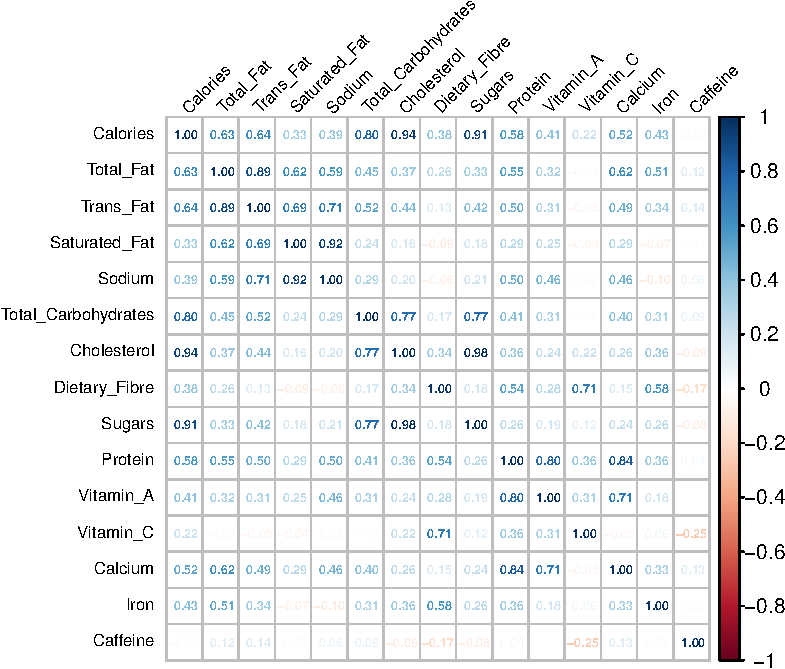
\includegraphics{Statistical_Learning_Final_Report_files/figure-latex/correlation_analysis-1} \end{center}

\section{Data Visualization}\label{data-visualization}

Data visualization is a powerful tool that allows us to uncover
patterns, correlations and outliers in our data. It provides visual
information on the dataset in our analysis, representing large amounts
of data in a clear and comprehensive way and underlining the
relationships among them. This enables us to recognize patterns quickly.

So, let us transform our raw data into graphical representations, to
gain a more comprehensive understanding of the information at hand.

\subsection{Histograms}\label{histograms}

Histograms serve as a graphical interpretation of data distribution. In
a histogram, each bar corresponds to the counted frequency within each
bin or interval. We introduce these plots to see if our data is normally
distributed, skewed, or has outlier values.

\begin{center}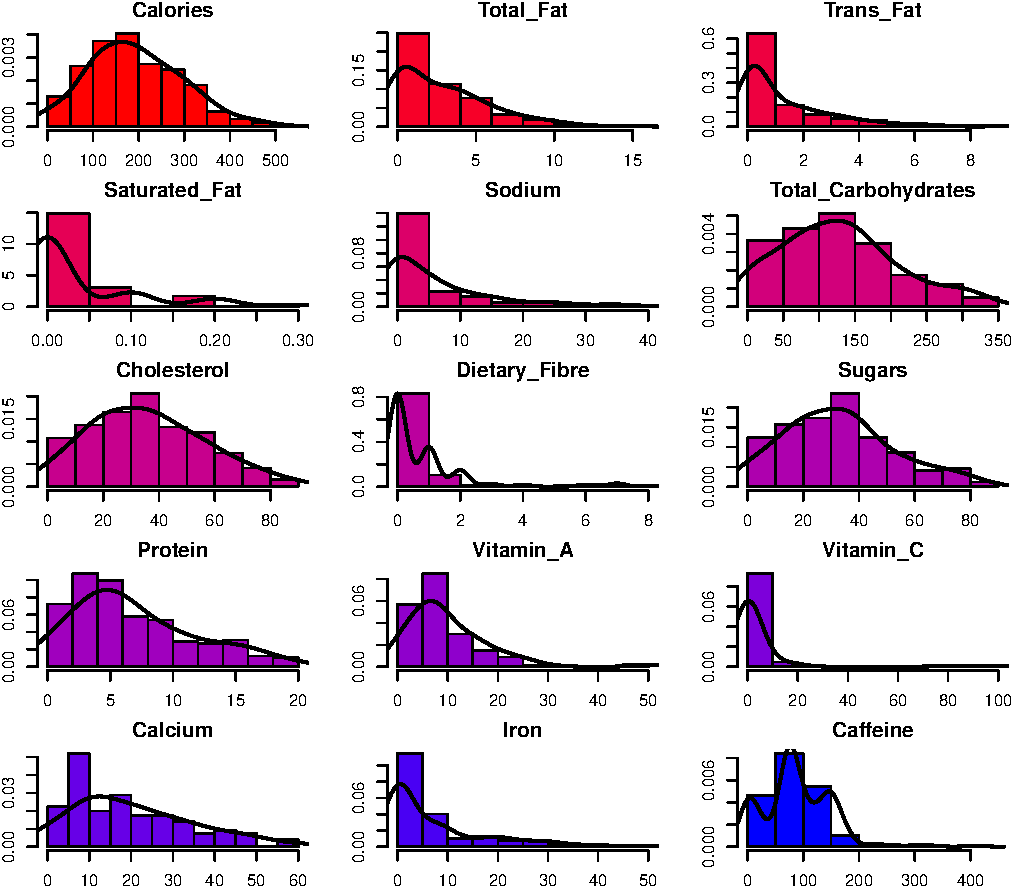
\includegraphics{Statistical_Learning_Final_Report_files/figure-latex/histograms-1} \end{center}

By looking at the graphs, we can notice that the variables
\texttt{"Calories"}, \texttt{"Total\_Carbohydrates"},
\texttt{"Cholesterol"}, and \texttt{"Sugars"} exhibit distributions that
are nearly normal. Conversely, the distributions of the remaining
variables display a noticeable skewness towards the left.

\subsection{Barplot}\label{barplot}

We will now plot the bar plots for our dataset. The primary use of bar
plots is to make comparisons between the amounts of different
categories. Indeed, each bar corresponds to a category and the height of
the bar represents the frequency or proportion of that category. These
graphs are commonly used for categorical data, or numerical data that
has been binned into categories.

\begin{center}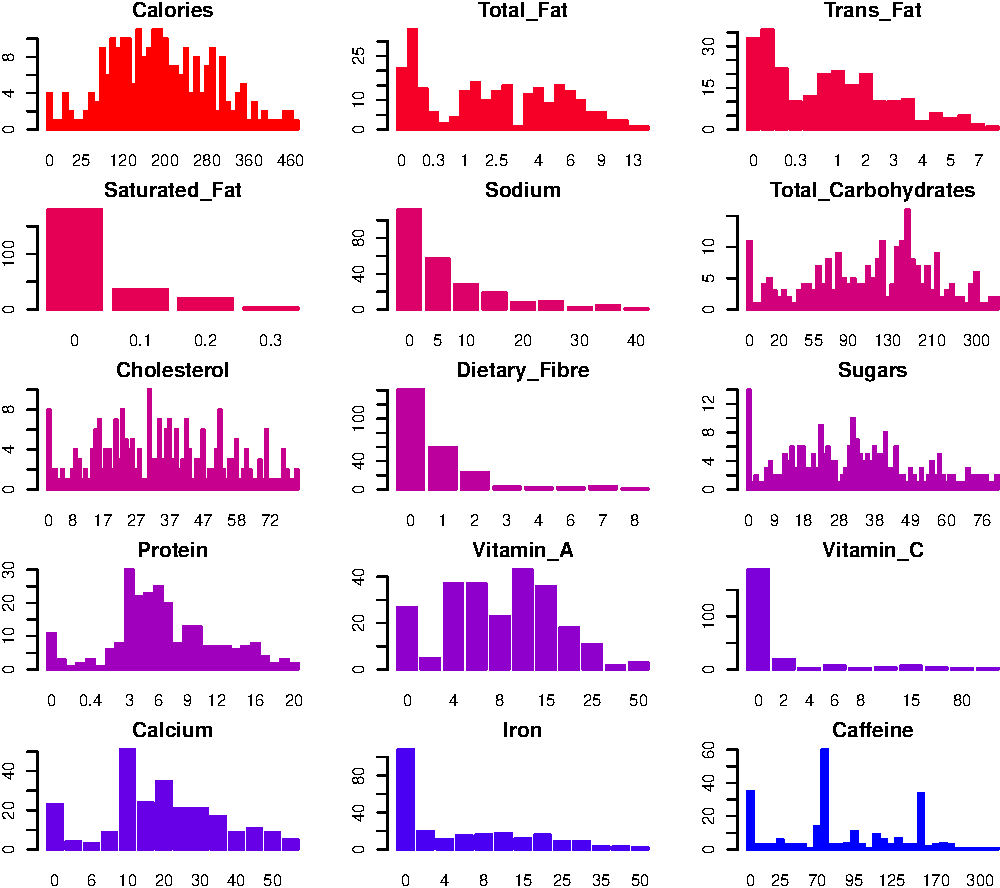
\includegraphics{Statistical_Learning_Final_Report_files/figure-latex/barplot-1} \end{center}

We can deduce some useful information by looking at these plots.

For example, we can notice that variables such as
\texttt{"Saturated\_Fat"}, \texttt{"Dietary\_Fibre"},
\texttt{"Vitamin\_C"}, and \texttt{"Iron"} are typically either absent
or present in small quantities in the beverages. In particular, the
frequency of these variables rapidly diminishes as their levels
increase. On the other hand, the variables \texttt{"Calories"},
\texttt{"Total\_Fat"}, \texttt{"Trans\_Fat"}, and
\texttt{"Total\_Carbohydrates"} show a wide range of values across
different beverage types, going from high levels in some beverages to
minimal amounts in others.

We can further observe that the distribution of \texttt{"Vitamin\_A"}
appears to be more evenly spread among the different levels in various
beverages, while instead \texttt{"Caffeine"} plot is interesting as it
exhibits three distinct peaks in frequency.

\subsection{Boxplot}\label{boxplot}

Boxplots are a type of graphical representation used to display the
distribution of a dataset. They provide a visual summary of the data,
enabling us to quickly identify key statistical measures such as median,
quartiles and outliers. This visualization also helps us to determine
the spread and variability of the data.

\begin{center}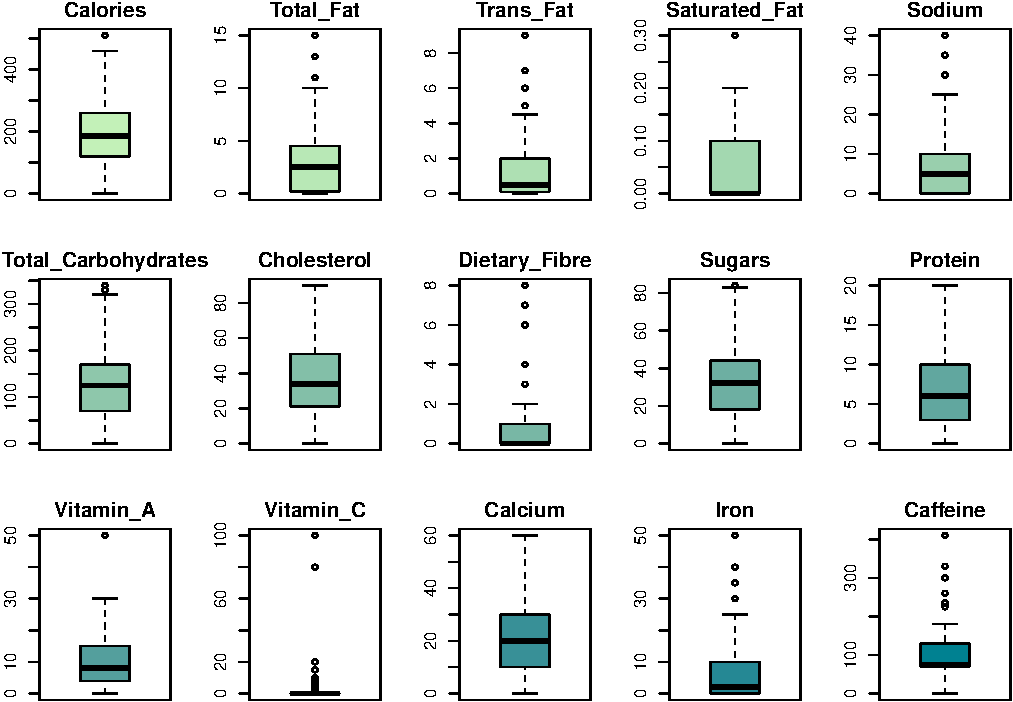
\includegraphics{Statistical_Learning_Final_Report_files/figure-latex/boxplot-1} \end{center}

As we observed earlier, the majority of the graphs exhibits a skewness
towards zero, with the exceptions being \texttt{“Calories”},
\texttt{“Total\_Carbohydrates”}, \texttt{“Cholesterol”}, and
\texttt{“Sugars”}.

Another aspect that has not been previously highlighted is the presence
of outliers. These are notably evident in \texttt{“Dietary\_Fiber”},
\texttt{“Vitamin\_C”}, and \texttt{“Caffeine”} plots.

\subsection{Scatterplot}\label{scatterplot}

A scatterplot is a type of data visualization that uses dots to
represent the values obtained for two different variables - one plotted
along the x-axis and the other plotted along the y-axis. Scatterplots
are used to observe relationships between variables. This type of
graphical representation is crucial in detecting underlying patterns and
potential correlations among the variables.

In particular, we place the calorie content and fat levels of various
beverage categories side by side for comparison. To make the
visualization more intuitive, we assign distinct colors to each beverage
category and create a legend to identify each category.

\begin{center}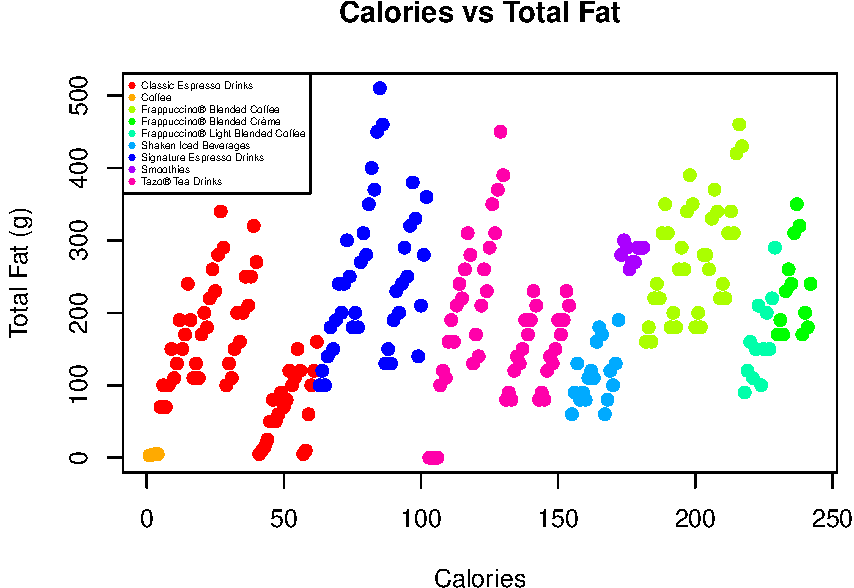
\includegraphics{Statistical_Learning_Final_Report_files/figure-latex/fat_comparison-1} \end{center}

Let us look for any overall pattern or trend in the data points. For all
the categories the two variables seem to be related following an almost
linear trend, with a positive correlation - as one variable increases,
so does the other. However, it is important to note that a very high
\texttt{"Total\_Fat"} value does not necessarily equate to a very high
\texttt{"Calories"} value - see \texttt{"Espresso\ Signature\ Drinks"}
category.

Additionally we can observe that, given a specific category, it is
possible that we find two clusters of data points that follow distinct
distibutions. This phenomenon is observed in the
\texttt{"Classic\ Espresso\ Drinks"},
\texttt{"Espresso\ Signature\ Drinks"} and \texttt{"Tazo\ Tea\ Drinks"}
categories and it is likely attributable to the diverse methods of drink
preparation.

Finally, we create some scatterplots to look into relantionship between
\texttt{"Calories"} and other variables. In particular we focus on
\texttt{"Sodium"}, \texttt{"Protein"}, \texttt{"Sugars"} and
\texttt{"Dietary\_Fiber"}.

\begin{center}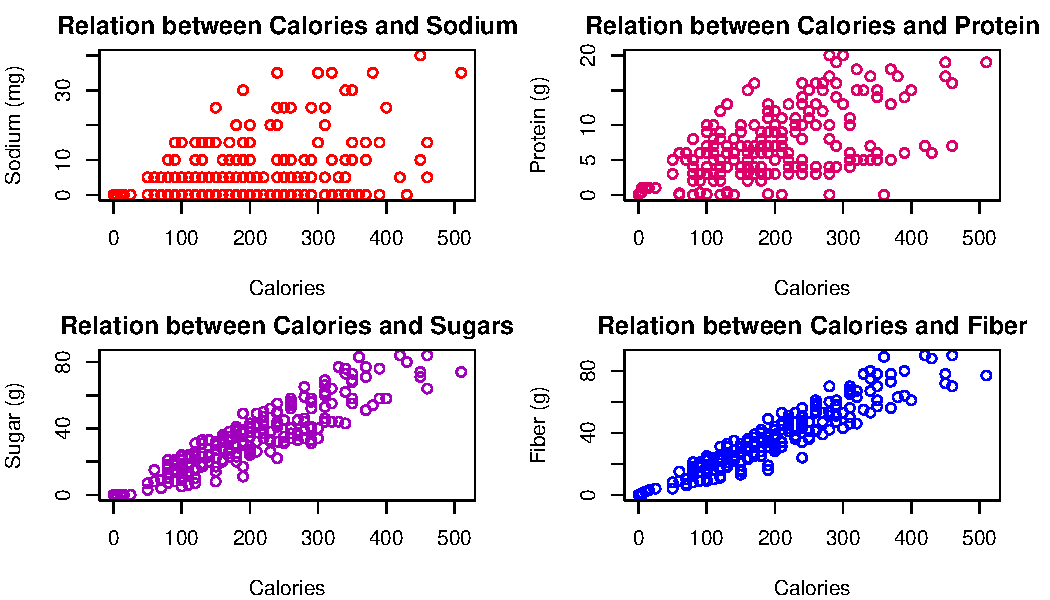
\includegraphics{Statistical_Learning_Final_Report_files/figure-latex/scatterplot-1} \end{center}

With an increase in calories, we observe a corresponding rise in all
features. However, the rate of increase varies among different features.
For instance, \texttt{"Sugars"} and \texttt{"Dietary\_Fiber"} show a
steep ascent, indicating a rapid increase with calorie count. On the
other hand, \texttt{"Sodium"} and \texttt{"Protein"} exhibit a more
gradual growth, suggesting a slower rate of increase despite the rising
calorie content. These observations are further substantiated by the
correlation coefficients, which provide a quantitative measure of these
relationships. This highlights the complex interplay between calories
and various nutritional components in our beverages.

\subsection{Pairplot}\label{pairplot}

A pairplot, as the name suggests, is a plot that enables us to visualize
the pairwise relationships between different variables in a dataset. It
is essentially a matrix of scatterplots, where each scatterplot shows
the relationship between a pair of variables. This type of visualization
is particularly useful for exploring potential relationships and
correlations between all the variables. As previously noted, by
examining the scatterplots we can identify patterns, trends, and
outliers in the data.

Before we can create a pairplot, we need to define a some functions for
it. This functions will generate the scatterplots, as well as additional
elements such as histograms, correlation coefficients, and a smooth line
to help visualize the distribution and correlation of the data.

Finally, we create the pairplot using the defined functions.

\begin{center}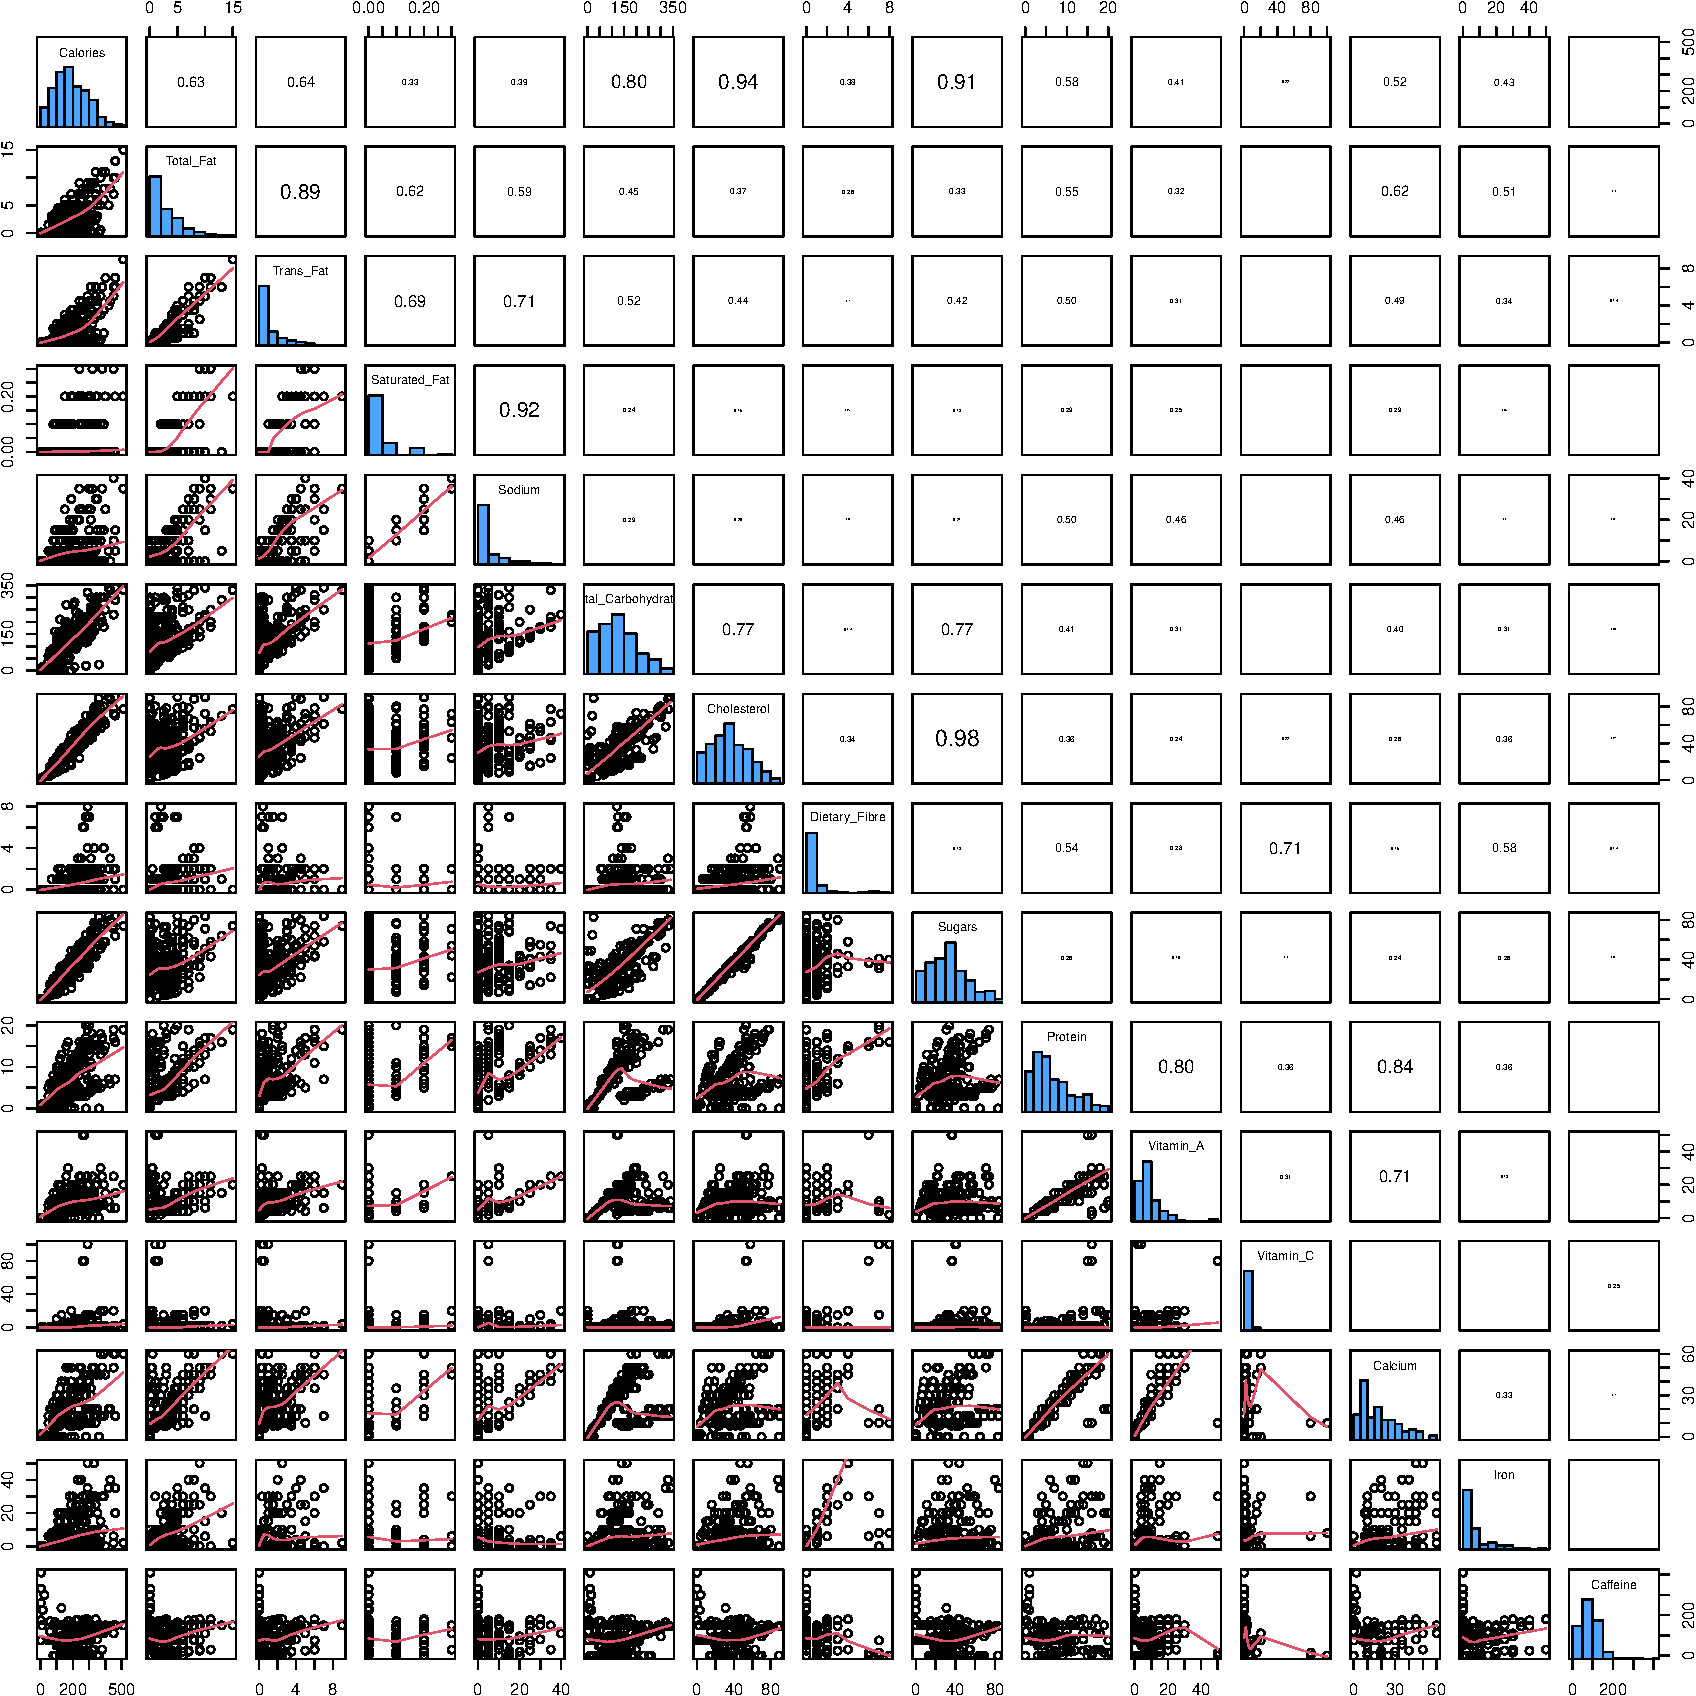
\includegraphics{Statistical_Learning_Final_Report_files/figure-latex/pairplot-1} \end{center}

\textbf{ADD COMMENTS ON THE GRAPH (I don't know how to comment it)}

\section{Regression Analysis}\label{regression-analysis}

In this section we will conduct a comprehensive regression analysis on
our dataset, exploring our data, constructing different models and
lastly performing model selection and validation. Our goal is to build a
model that accurately represents the relationships within our data and
can provide meaningful predictions. In particular, the variable we want
to predict is \texttt{"Calories"}. To achieve this, we will first fit a
linear regression model to predict the amount of calories based on the
amount of the other variables. We will then compare different models,
evaluate their performance, and select the best model for our data.

\subsection{Linear Regression}\label{linear-regression}

The simplest form of regression analysis is linear regression, where we
predict an outcome variable based on one or more predictor variables.

Linear regression model to predict the amount of calories based on the
amount of the other variables We use the \texttt{lm()} function to fit a
linear regression model to predict the amount of calories based on the
amount of the other variables in the dataset. We then evaluate the model
using various metrics such as AIC, BIC, R-squared, and adjusted
R-squared.

\subsubsection{Simple Linear Regression}\label{simple-linear-regression}

Fit linear simple regression with just one variable on
\texttt{data\_cleaned}, looking at correlation plot we choose
\texttt{Sugars} due to high correlation.

This code will fit a simple linear regression model predicting
\texttt{"Calories"} using \texttt{"Sugars"} as the predictor variable
and provide a summary of the model.

\begin{Shaded}
\begin{Highlighting}[]
\NormalTok{lm\_simple }\OtherTok{\textless{}{-}} \FunctionTok{lm}\NormalTok{(Calories }\SpecialCharTok{\textasciitilde{}}\NormalTok{ Sugars, }\AttributeTok{data =}\NormalTok{ data\_cleaned)}
\FunctionTok{kable}\NormalTok{(}\FunctionTok{data.frame}\NormalTok{(}\AttributeTok{AIC =} \FunctionTok{AIC}\NormalTok{(lm\_simple), }\AttributeTok{BIC =} \FunctionTok{BIC}\NormalTok{(lm\_simple),}
                 \AttributeTok{R\_squared =} \FunctionTok{summary}\NormalTok{(lm\_simple)}\SpecialCharTok{$}\NormalTok{r.squared, }
                 \AttributeTok{adj\_R\_squared =} \FunctionTok{summary}\NormalTok{(lm\_simple)}\SpecialCharTok{$}\NormalTok{adj.r.squared), }
      \AttributeTok{caption =} \StringTok{"Model evaluation metrics for the simple linear regression model"}\NormalTok{)}
\end{Highlighting}
\end{Shaded}

\begin{longtable}[]{@{}rrrr@{}}
\caption{Model evaluation metrics for the simple linear regression
model}\tabularnewline
\toprule\noalign{}
AIC & BIC & R\_squared & adj\_R\_squared \\
\midrule\noalign{}
\endfirsthead
\toprule\noalign{}
AIC & BIC & R\_squared & adj\_R\_squared \\
\midrule\noalign{}
\endhead
\bottomrule\noalign{}
\endlastfoot
2509.036 & 2519.503 & 0.8275094 & 0.8267907 \\
\end{longtable}

\begin{Shaded}
\begin{Highlighting}[]
\FunctionTok{par}\NormalTok{(}\AttributeTok{mfrow =} \FunctionTok{c}\NormalTok{(}\DecValTok{2}\NormalTok{, }\DecValTok{2}\NormalTok{), }\AttributeTok{mar =} \FunctionTok{c}\NormalTok{(}\DecValTok{2}\NormalTok{, }\DecValTok{2}\NormalTok{, }\DecValTok{2}\NormalTok{, }\DecValTok{2}\NormalTok{))}
\FunctionTok{plot}\NormalTok{(lm\_simple)}
\end{Highlighting}
\end{Shaded}

\begin{center}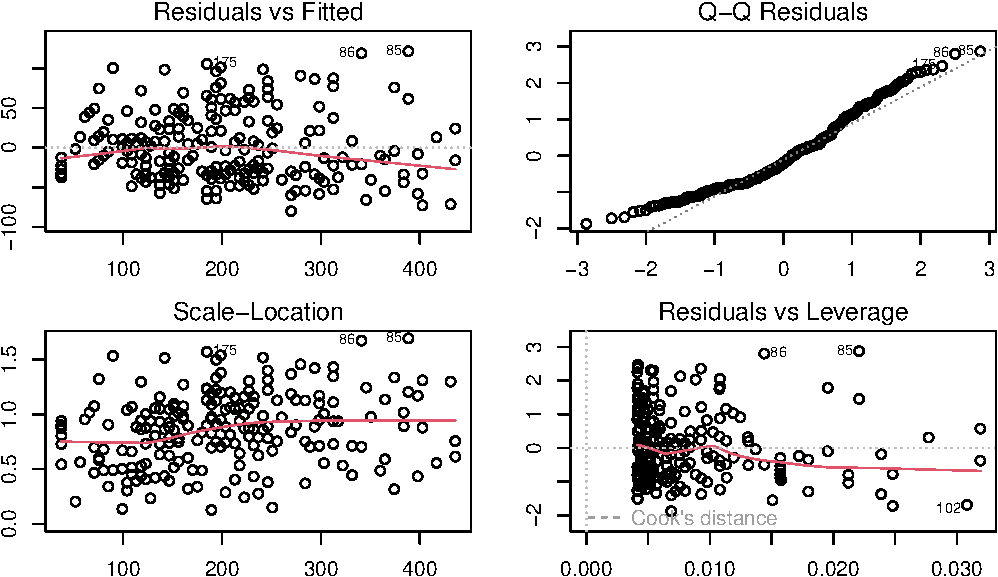
\includegraphics{Statistical_Learning_Final_Report_files/figure-latex/simple_linear_regression-1} \end{center}

The coefficient for \texttt{"Sugars"} (\(4.7426\)) indicates that, on
average, for every one-unit increase in \texttt{"Sugars"}, the predicted
\texttt{"Calories"} increases by approximately \(4.7426\) units. Both
the intercept and the coefficient for \texttt{"Sugars"} are
statistically significant (\(p < 0.001\)), indicating a strong linear
relationship between \texttt{"Sugars"} and \texttt{"Calories"}. The
F-statistic is highly significant (\(p < 2.2e-16\)), indicating that the
overall regression model is statistically significant in explaining the
variance in \texttt{"Calories"}. Model Fit:The adjusted R-squared value
(\(0.8268\)) indicates that approximately \(82.68\)\% of the variance in
\texttt{"Calories"} can be explained by the predictor variable
\texttt{"Sugars"}. Overall, this output suggests that the simple linear
regression model provides a statistically significant relationship
between \texttt{"Sugars"} and \texttt{"Calories"}, with
\texttt{"Sugars"} being a strong predictor of \texttt{"Calories"}.
However, the AIC and BIC values suggest that there might be other models
that provide a better fit for the data.

Summarizing the model is too simple so it doesn't capture the complexity
of the data, so we try to fit a multiple linear regression model.

\subsubsection{Multiple Linear
Regression}\label{multiple-linear-regression}

\begin{Shaded}
\begin{Highlighting}[]
\NormalTok{lm\_model }\OtherTok{\textless{}{-}} \FunctionTok{lm}\NormalTok{(y }\SpecialCharTok{\textasciitilde{}}\NormalTok{ ., }\AttributeTok{data =}\NormalTok{ data\_num\_)}
\FunctionTok{par}\NormalTok{(}\AttributeTok{mfrow =} \FunctionTok{c}\NormalTok{(}\DecValTok{2}\NormalTok{, }\DecValTok{2}\NormalTok{), }\AttributeTok{mar =} \FunctionTok{c}\NormalTok{(}\DecValTok{2}\NormalTok{, }\DecValTok{2}\NormalTok{, }\DecValTok{2}\NormalTok{, }\DecValTok{2}\NormalTok{))}
\FunctionTok{plot}\NormalTok{(lm\_model)}
\end{Highlighting}
\end{Shaded}

\begin{center}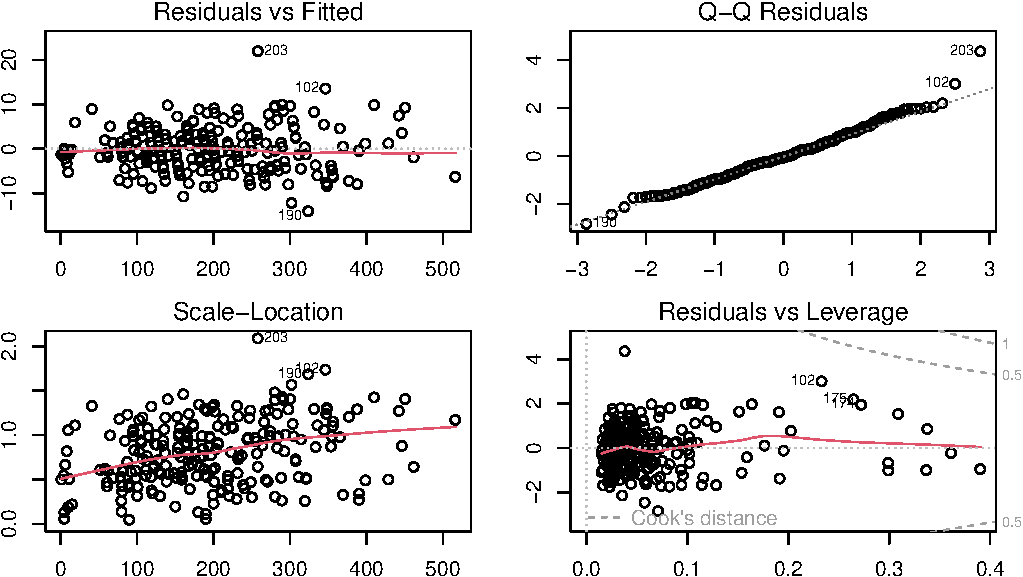
\includegraphics{Statistical_Learning_Final_Report_files/figure-latex/multiple_linear_regression-1} \end{center}

\begin{Shaded}
\begin{Highlighting}[]
\FunctionTok{kable}\NormalTok{(}\FunctionTok{data.frame}\NormalTok{(}\AttributeTok{AIC =} \FunctionTok{AIC}\NormalTok{(lm\_model), }\AttributeTok{BIC =} \FunctionTok{BIC}\NormalTok{(lm\_model),}
                 \AttributeTok{R\_squared =} \FunctionTok{summary}\NormalTok{(lm\_model)}\SpecialCharTok{$}\NormalTok{r.squared, }
                 \AttributeTok{adj\_R\_squared =} \FunctionTok{summary}\NormalTok{(lm\_model)}\SpecialCharTok{$}\NormalTok{adj.r.squared),}
      \AttributeTok{caption =} \StringTok{"Model evaluation metrics for the linear regression model"}\NormalTok{)}
\end{Highlighting}
\end{Shaded}

\begin{longtable}[]{@{}rrrr@{}}
\caption{Model evaluation metrics for the linear regression
model}\tabularnewline
\toprule\noalign{}
AIC & BIC & R\_squared & adj\_R\_squared \\
\midrule\noalign{}
\endfirsthead
\toprule\noalign{}
AIC & BIC & R\_squared & adj\_R\_squared \\
\midrule\noalign{}
\endhead
\bottomrule\noalign{}
\endlastfoot
1494.304 & 1550.127 & 0.9976608 & 0.9975166 \\
\end{longtable}

The model has a low AIC and BIC values, the R-squared value is \(0.997\)
so the model is a good fit for the data.

\subsubsection{Backward Elimination}\label{backward-elimination}

Now we apply the selection of the predictors with the backward
elimination method. This method starts with all the predictors in the
model and then removes the least significant predictor one at a time
until all remaining predictors are significant.

\begin{Shaded}
\begin{Highlighting}[]
\FunctionTok{par}\NormalTok{(}\AttributeTok{mfrow =} \FunctionTok{c}\NormalTok{(}\DecValTok{2}\NormalTok{, }\DecValTok{2}\NormalTok{), }\AttributeTok{mar =} \FunctionTok{c}\NormalTok{(}\DecValTok{2}\NormalTok{, }\DecValTok{2}\NormalTok{, }\DecValTok{2}\NormalTok{, }\DecValTok{2}\NormalTok{))}
\FunctionTok{plot}\NormalTok{(backward\_model)}
\end{Highlighting}
\end{Shaded}

\begin{center}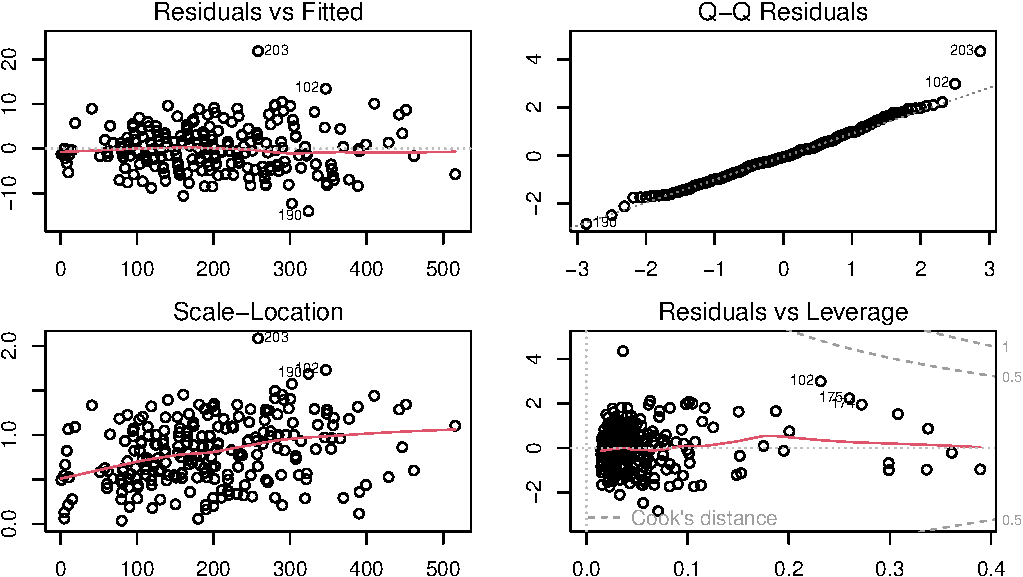
\includegraphics{Statistical_Learning_Final_Report_files/figure-latex/backward_elimination-1} \end{center}

\begin{Shaded}
\begin{Highlighting}[]
\FunctionTok{kable}\NormalTok{(}\FunctionTok{data.frame}\NormalTok{(}\AttributeTok{AIC =} \FunctionTok{AIC}\NormalTok{(backward\_model), }\AttributeTok{BIC =} \FunctionTok{BIC}\NormalTok{(backward\_model),}
                 \AttributeTok{R\_squared =} \FunctionTok{summary}\NormalTok{(backward\_model)}\SpecialCharTok{$}\NormalTok{r.squared, }
                 \AttributeTok{adj\_R\_squared =} \FunctionTok{summary}\NormalTok{(backward\_model)}\SpecialCharTok{$}\NormalTok{adj.r.squared),}
      \AttributeTok{caption =} \StringTok{"Model evaluation metrics for the linear regression model }
\StringTok{      with backward elimination"}\NormalTok{)}
\end{Highlighting}
\end{Shaded}

\begin{longtable}[]{@{}rrrr@{}}
\caption{Model evaluation metrics for the linear regression model with
backward elimination}\tabularnewline
\toprule\noalign{}
AIC & BIC & R\_squared & adj\_R\_squared \\
\midrule\noalign{}
\endfirsthead
\toprule\noalign{}
AIC & BIC & R\_squared & adj\_R\_squared \\
\midrule\noalign{}
\endhead
\bottomrule\noalign{}
\endlastfoot
1492.616 & 1544.95 & 0.9976578 & 0.9975243 \\
\end{longtable}

The backward selection drops only the variable \texttt{"Saturated\_Fat"}
since it's not considered significant in explaining the amount of
calories mantaining the other variables.

\textbf{Comarison between the models:}

\begin{longtable}[]{@{}
  >{\raggedright\arraybackslash}p{(\columnwidth - 8\tabcolsep) * \real{0.5579}}
  >{\raggedleft\arraybackslash}p{(\columnwidth - 8\tabcolsep) * \real{0.0947}}
  >{\raggedleft\arraybackslash}p{(\columnwidth - 8\tabcolsep) * \real{0.0947}}
  >{\raggedleft\arraybackslash}p{(\columnwidth - 8\tabcolsep) * \real{0.1053}}
  >{\raggedleft\arraybackslash}p{(\columnwidth - 8\tabcolsep) * \real{0.1474}}@{}}
\caption{Model comparison}\tabularnewline
\toprule\noalign{}
\begin{minipage}[b]{\linewidth}\raggedright
Model
\end{minipage} & \begin{minipage}[b]{\linewidth}\raggedleft
AIC
\end{minipage} & \begin{minipage}[b]{\linewidth}\raggedleft
BIC
\end{minipage} & \begin{minipage}[b]{\linewidth}\raggedleft
R\_squared
\end{minipage} & \begin{minipage}[b]{\linewidth}\raggedleft
adj\_R\_squared
\end{minipage} \\
\midrule\noalign{}
\endfirsthead
\toprule\noalign{}
\begin{minipage}[b]{\linewidth}\raggedright
Model
\end{minipage} & \begin{minipage}[b]{\linewidth}\raggedleft
AIC
\end{minipage} & \begin{minipage}[b]{\linewidth}\raggedleft
BIC
\end{minipage} & \begin{minipage}[b]{\linewidth}\raggedleft
R\_squared
\end{minipage} & \begin{minipage}[b]{\linewidth}\raggedleft
adj\_R\_squared
\end{minipage} \\
\midrule\noalign{}
\endhead
\bottomrule\noalign{}
\endlastfoot
Simple Linear Regression & 2509.036 & 2519.503 & 0.8275094 &
0.8267907 \\
Multiple Linear Regression & 1494.304 & 1550.127 & 0.9976608 &
0.9975166 \\
Multiple Linear Regression with Backward Elimination & 1492.616 &
1544.950 & 0.9976578 & 0.9975243 \\
\end{longtable}

The multiple linear regression model with backward elimination has the
lowest AIC and BIC values, the highest R-squared value, and the highest
adjusted R-squared value, indicating that it is the best model for
predicting the amount of calories based on the amount of the other
variables.

\textbf{Coefficients:} Both models have very similar coefficients for
the variables that were retained. The removal of
\texttt{"Saturated\_Fat"} in the backward model did not significantly
affect the estimates of the other coefficients.

\textbf{Significance of Variables:} In the full model,
\texttt{"Saturated\_Fat"} had a high p-value (\(0.589\)), indicating it
was not a significant variable. In the backward model,
\texttt{"Saturated\_Fat"} was removed, slightly improving the AIC while
keeping all other variables significant.

\textbf{Overall Performance:} Both models perform very similarly in
terms of R-squared and residual standard error. The backward model is
preferable because it has a slightly lower AIC, suggesting it is a more
parsimonious model without sacrificing the quality of the fit.

\subsubsection{Anova}\label{anova}

Anova comparison between the models

\begin{Shaded}
\begin{Highlighting}[]
\NormalTok{anova\_results }\OtherTok{\textless{}{-}} \FunctionTok{anova}\NormalTok{(lm\_model, backward\_model)}
\NormalTok{anova\_results}
\end{Highlighting}
\end{Shaded}

\begin{verbatim}
## Analysis of Variance Table
## 
## Model 1: y ~ Total_Fat + Trans_Fat + Saturated_Fat + Sodium + Total_Carbohydrates + 
##     Cholesterol + Dietary_Fibre + Sugars + Protein + Vitamin_A + 
##     Vitamin_C + Calcium + Iron + Caffeine
## Model 2: y ~ Total_Fat + Trans_Fat + Sodium + Total_Carbohydrates + Cholesterol + 
##     Dietary_Fibre + Sugars + Protein + Vitamin_A + Vitamin_C + 
##     Calcium + Iron + Caffeine
##   Res.Df    RSS Df Sum of Sq      F Pr(>F)
## 1    227 5964.8                           
## 2    228 5972.5 -1   -7.6917 0.2927  0.589
\end{verbatim}

\textbf{Degrees of Freedom (Res.Df):} The full model has \(227\) degrees
of freedom, while the backward model has \(228\). This is because we
removed one variable from the full model.

\textbf{Residual Sum of Squares (RSS):} The full model has an RSS of
\(5964.83\), while the backward model has an RSS of \(5972.55\). This
indicates that the difference between the two models in terms of
residual error is very small.

\textbf{Sum of Squares (Sum of Sq):} The difference between the two
models in terms of sum of squares is \(-7.7235\), indicating that the
removed variable (\texttt{"Saturated\_Fat"}) does not significantly
contribute to explaining the variability in calories.

\textbf{F-statistic (F):} The F value is \(0.2937\) with a p-value of
\(0.588\). This high p-value indicates that there is no significant
difference between the two models. In other words, the reduced model is
not significantly worse than the full model.

\textbf{Conclusion:} The ANOVA shows that the removal of the
\texttt{"Saturated\_Fat"} variable does not have a significant impact on
the model. This confirms that the model obtained through backward
selection is more parsimonious without compromising the quality of the
fit. Therefore, the backward model is preferable to the full model.

\subsubsection{Multicollinearity}\label{multicollinearity}

To check for multicollinearity, we calculate the Variance Inflation
Factors (VIF) for the variables in the multiple linear regression model,
it measures how much the variance of the estimated coefficients is
increased due to multicollinearity.Usually a VIF value greater than
\(10\) indicates a problematic amount of multicollinearity.

\begin{longtable}[]{@{}lr@{}}
\caption{VIF values for the linear regression model}\tabularnewline
\toprule\noalign{}
& VIF \\
\midrule\noalign{}
\endfirsthead
\toprule\noalign{}
& VIF \\
\midrule\noalign{}
\endhead
\bottomrule\noalign{}
\endlastfoot
Total\_Fat & 17.863697 \\
Trans\_Fat & 14.667324 \\
Sodium & 4.448925 \\
Total\_Carbohydrates & 3.419094 \\
Cholesterol & 442.886703 \\
Dietary\_Fibre & 16.896773 \\
Sugars & 417.769822 \\
Protein & 56.706156 \\
Vitamin\_A & 4.205667 \\
Vitamin\_C & 4.288442 \\
Calcium & 37.105615 \\
Iron & 5.027804 \\
Caffeine & 1.176323 \\
\end{longtable}

However as we can see from the \emph{Table X} e have a problem with
multicollinearity, the VIF values are high for some variables, so we
have to act on the data to solve this problem

The high values of the VIF could be due to:

\begin{itemize}
\item
  High correlation between variables,means that variable contribuite in
  the same way to predict and explain calories
\item
  Same information
\item
  Data unbalanced
\item
  Different Measurement Scales: If the variables in the model have
  significantly different measurement scales such as g and mg this could
  affect the VIF values.
\item
  Non-linear Relationships: If the relationships between the variables
  are non-linear, this could also affect the VIF values.
\end{itemize}

In this case, normalizing the variables might help reduce
multicollinearity.

\subsubsection{Standardize the data}\label{standardize-the-data}

We have tried different kind of standardization to reduce the
multicollinearity First at all we tried the scale by standard
normalization The negative value of the AIC (\(-748.2623\)) indicates
that the standardized linear regression model provides a better
compromise between data fit and model complexity compared to the
reference model. However, the VIF values are still high, indicating that
multicollinearity is still present in the model.

To reduce the problem of high VIF in linear regression, it is generally
preferable to use the transformation that includes both log
transformation and standardization of the data. This is because
standardization helps to put all variables on the same scale, reducing
the likelihood of multicollinearity. Log transformation: Reduces the
variance of the variables, making the distribution more normal and
reducing the impact of outliers. Standardization: Puts all variables on
a common scale, with mean \(0\) and standard deviation \(1\), further
reducing multicollinearity.

\begin{Shaded}
\begin{Highlighting}[]
\NormalTok{std\_data\_log }\OtherTok{\textless{}{-}} \FunctionTok{scale}\NormalTok{(}\FunctionTok{log}\NormalTok{(data\_num }\SpecialCharTok{+} \DecValTok{1}\NormalTok{)) }\CommentTok{\# Standardize the data}
\NormalTok{std\_data\_log\_df }\OtherTok{\textless{}{-}} \FunctionTok{as.data.frame}\NormalTok{(std\_data\_log) }\CommentTok{\# Set as dataframe}
\NormalTok{mod\_log\_tr }\OtherTok{\textless{}{-}} \FunctionTok{lm}\NormalTok{(Calories }\SpecialCharTok{\textasciitilde{}}\NormalTok{ ., }\AttributeTok{data =}\NormalTok{ std\_data\_log\_df)}
\FunctionTok{kable}\NormalTok{(}\FunctionTok{data.frame}\NormalTok{(}\AttributeTok{AIC =} \FunctionTok{AIC}\NormalTok{(mod\_log\_tr), }\AttributeTok{BIC =} \FunctionTok{BIC}\NormalTok{(mod\_log\_tr),}
                 \AttributeTok{R\_squared =} \FunctionTok{summary}\NormalTok{(mod\_log\_tr)}\SpecialCharTok{$}\NormalTok{r.squared, }
                 \AttributeTok{adj\_R\_squared =} \FunctionTok{summary}\NormalTok{(mod\_log\_tr)}\SpecialCharTok{$}\NormalTok{adj.r.squared), }
      \AttributeTok{caption =} \StringTok{"Model evaluation metrics for the log transformed data"}\NormalTok{)}
\end{Highlighting}
\end{Shaded}

\begin{longtable}[]{@{}rrrr@{}}
\caption{Model evaluation metrics for the log transformed
data}\tabularnewline
\toprule\noalign{}
AIC & BIC & R\_squared & adj\_R\_squared \\
\midrule\noalign{}
\endfirsthead
\toprule\noalign{}
AIC & BIC & R\_squared & adj\_R\_squared \\
\midrule\noalign{}
\endhead
\bottomrule\noalign{}
\endlastfoot
-53.42411 & 2.398897 & 0.9586932 & 0.9561457 \\
\end{longtable}

\begin{Shaded}
\begin{Highlighting}[]
\FunctionTok{kable}\NormalTok{(}\FunctionTok{data.frame}\NormalTok{(}\AttributeTok{VIF =} \FunctionTok{vif}\NormalTok{(mod\_log\_tr)),}
      \AttributeTok{caption =} \StringTok{"VIF values for the log transformed data"}\NormalTok{)}
\end{Highlighting}
\end{Shaded}

\begin{longtable}[]{@{}lr@{}}
\caption{VIF values for the log transformed data}\tabularnewline
\toprule\noalign{}
& VIF \\
\midrule\noalign{}
\endfirsthead
\toprule\noalign{}
& VIF \\
\midrule\noalign{}
\endhead
\bottomrule\noalign{}
\endlastfoot
Total\_Fat & 12.049669 \\
Trans\_Fat & 10.577306 \\
Saturated\_Fat & 4.528080 \\
Sodium & 5.817088 \\
Total\_Carbohydrates & 4.363628 \\
Cholesterol & 39.988684 \\
Dietary\_Fibre & 7.115085 \\
Sugars & 38.415586 \\
Protein & 31.007121 \\
Vitamin\_A & 13.647581 \\
Vitamin\_C & 2.196674 \\
Calcium & 25.873742 \\
Iron & 4.582594 \\
Caffeine & 1.310005 \\
\end{longtable}

\begin{Shaded}
\begin{Highlighting}[]
\FunctionTok{par}\NormalTok{(}\AttributeTok{mfrow =} \FunctionTok{c}\NormalTok{(}\DecValTok{2}\NormalTok{, }\DecValTok{2}\NormalTok{), }\AttributeTok{mar =} \FunctionTok{c}\NormalTok{(}\DecValTok{2}\NormalTok{, }\DecValTok{2}\NormalTok{, }\DecValTok{2}\NormalTok{, }\DecValTok{2}\NormalTok{))}
\FunctionTok{plot}\NormalTok{(mod\_log\_tr)}
\end{Highlighting}
\end{Shaded}

\begin{center}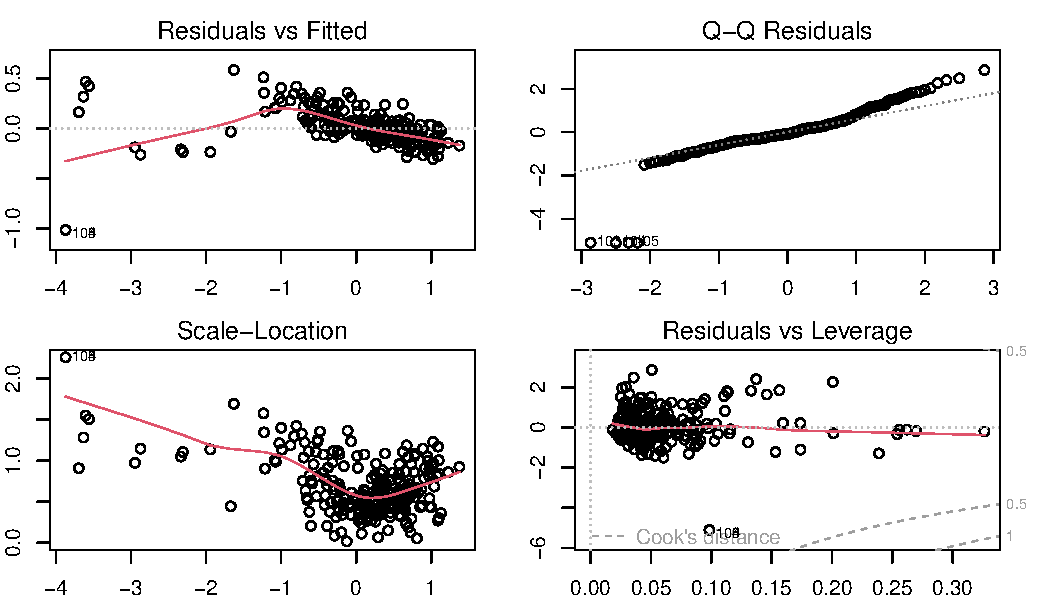
\includegraphics{Statistical_Learning_Final_Report_files/figure-latex/standardization-1} \end{center}

The model has a low AIC and BIC values, the R-squared value is \(0.95\)
so the model is a good fit for the data. However we have still
collinearity, so we try to use backward elimination to check if this
method will removes the variables that are not significant in the model.

\begin{Shaded}
\begin{Highlighting}[]
\FunctionTok{kable}\NormalTok{(}\FunctionTok{data.frame}\NormalTok{(}\AttributeTok{AIC =} \FunctionTok{AIC}\NormalTok{(backward\_model\_log), }\AttributeTok{BIC =} \FunctionTok{BIC}\NormalTok{(backward\_model\_log),}
                 \AttributeTok{R\_squared =} \FunctionTok{summary}\NormalTok{(backward\_model\_log)}\SpecialCharTok{$}\NormalTok{r.squared, }
                 \AttributeTok{adj\_R\_squared =} \FunctionTok{summary}\NormalTok{(backward\_model\_log)}\SpecialCharTok{$}\NormalTok{adj.r.squared), }
      \AttributeTok{caption =} \StringTok{"Model evaluation metrics for the log transformed data }
\StringTok{      with backward elimination"}\NormalTok{)}
\end{Highlighting}
\end{Shaded}

\begin{longtable}[]{@{}rrrr@{}}
\caption{Model evaluation metrics for the log transformed data with
backward elimination}\tabularnewline
\toprule\noalign{}
AIC & BIC & R\_squared & adj\_R\_squared \\
\midrule\noalign{}
\endfirsthead
\toprule\noalign{}
AIC & BIC & R\_squared & adj\_R\_squared \\
\midrule\noalign{}
\endhead
\bottomrule\noalign{}
\endlastfoot
-63.78109 & -32.38065 & 0.9580667 & 0.9568123 \\
\end{longtable}

\begin{Shaded}
\begin{Highlighting}[]
\FunctionTok{kable}\NormalTok{(}\FunctionTok{data.frame}\NormalTok{(}\AttributeTok{VIF =} \FunctionTok{vif}\NormalTok{(backward\_model\_log)),}
      \AttributeTok{caption =} \StringTok{"VIF values for the log transformed data with backward elimination"}\NormalTok{)}
\end{Highlighting}
\end{Shaded}

\begin{longtable}[]{@{}lr@{}}
\caption{VIF values for the log transformed data with backward
elimination}\tabularnewline
\toprule\noalign{}
& VIF \\
\midrule\noalign{}
\endfirsthead
\toprule\noalign{}
& VIF \\
\midrule\noalign{}
\endhead
\bottomrule\noalign{}
\endlastfoot
Total\_Fat & 5.823786 \\
Trans\_Fat & 5.161252 \\
Total\_Carbohydrates & 3.390622 \\
Cholesterol & 36.628698 \\
Dietary\_Fibre & 1.851534 \\
Sugars & 33.948827 \\
Protein & 2.976444 \\
\end{longtable}

AIC slightly worst and the VIF values are still high, indicating that
multicollinearity is still present in the model. So we try to remove
manually the variables that has high VIF values.

\begin{Shaded}
\begin{Highlighting}[]
\NormalTok{mod\_log\_tr\_updated }\OtherTok{\textless{}{-}} \FunctionTok{lm}\NormalTok{(Calories }\SpecialCharTok{\textasciitilde{}}\NormalTok{ . }\SpecialCharTok{{-}}\NormalTok{ Cholesterol }\SpecialCharTok{{-}}\NormalTok{ Sugars,}
                         \AttributeTok{data =}\NormalTok{ std\_data\_log\_df)}
\FunctionTok{kable}\NormalTok{(}\FunctionTok{data.frame}\NormalTok{(}\AttributeTok{VIF =} \FunctionTok{vif}\NormalTok{(mod\_log\_tr\_updated)),}
      \AttributeTok{caption =} \StringTok{"VIF values for the log transformed data with }
\StringTok{      manual removal of variables"}\NormalTok{)}
\end{Highlighting}
\end{Shaded}

\begin{longtable}[]{@{}lr@{}}
\caption{VIF values for the log transformed data with manual removal of
variables}\tabularnewline
\toprule\noalign{}
& VIF \\
\midrule\noalign{}
\endfirsthead
\toprule\noalign{}
& VIF \\
\midrule\noalign{}
\endhead
\bottomrule\noalign{}
\endlastfoot
Total\_Fat & 11.902918 \\
Trans\_Fat & 10.114112 \\
Saturated\_Fat & 4.466975 \\
Sodium & 5.782843 \\
Total\_Carbohydrates & 3.375194 \\
Dietary\_Fibre & 7.080360 \\
Protein & 26.902392 \\
Vitamin\_A & 12.396739 \\
Vitamin\_C & 1.985799 \\
Calcium & 25.519022 \\
Iron & 4.521552 \\
Caffeine & 1.295121 \\
\end{longtable}

\begin{Shaded}
\begin{Highlighting}[]
\FunctionTok{kable}\NormalTok{(}\FunctionTok{data.frame}\NormalTok{(}\AttributeTok{AIC =} \FunctionTok{AIC}\NormalTok{(mod\_log\_tr\_backward\_2), }\AttributeTok{BIC =} \FunctionTok{BIC}\NormalTok{(mod\_log\_tr\_backward\_2),}
                 \AttributeTok{R\_squared =} \FunctionTok{summary}\NormalTok{(mod\_log\_tr\_backward\_2)}\SpecialCharTok{$}\NormalTok{r.squared, }
                 \AttributeTok{adj\_R\_squared =} \FunctionTok{summary}\NormalTok{(mod\_log\_tr\_backward\_2)}\SpecialCharTok{$}\NormalTok{adj.r.squared), }
      \AttributeTok{caption =} \StringTok{"Model evaluation metrics for the log transformed data with}
\StringTok{      backward elimination and manual removal of variables"}\NormalTok{)}
\end{Highlighting}
\end{Shaded}

\begin{longtable}[]{@{}rrrr@{}}
\caption{Model evaluation metrics for the log transformed data with
backward elimination and manual removal of variables}\tabularnewline
\toprule\noalign{}
AIC & BIC & R\_squared & adj\_R\_squared \\
\midrule\noalign{}
\endfirsthead
\toprule\noalign{}
AIC & BIC & R\_squared & adj\_R\_squared \\
\midrule\noalign{}
\endhead
\bottomrule\noalign{}
\endlastfoot
460.5536 & 488.4651 & 0.6309185 & 0.6214952 \\
\end{longtable}

\begin{Shaded}
\begin{Highlighting}[]
\FunctionTok{par}\NormalTok{(}\AttributeTok{mfrow =} \FunctionTok{c}\NormalTok{(}\DecValTok{2}\NormalTok{, }\DecValTok{2}\NormalTok{), }\AttributeTok{mar =} \FunctionTok{c}\NormalTok{(}\DecValTok{2}\NormalTok{, }\DecValTok{2}\NormalTok{, }\DecValTok{2}\NormalTok{, }\DecValTok{2}\NormalTok{))}
\FunctionTok{plot}\NormalTok{(mod\_log\_tr\_backward\_2)}
\end{Highlighting}
\end{Shaded}

\begin{center}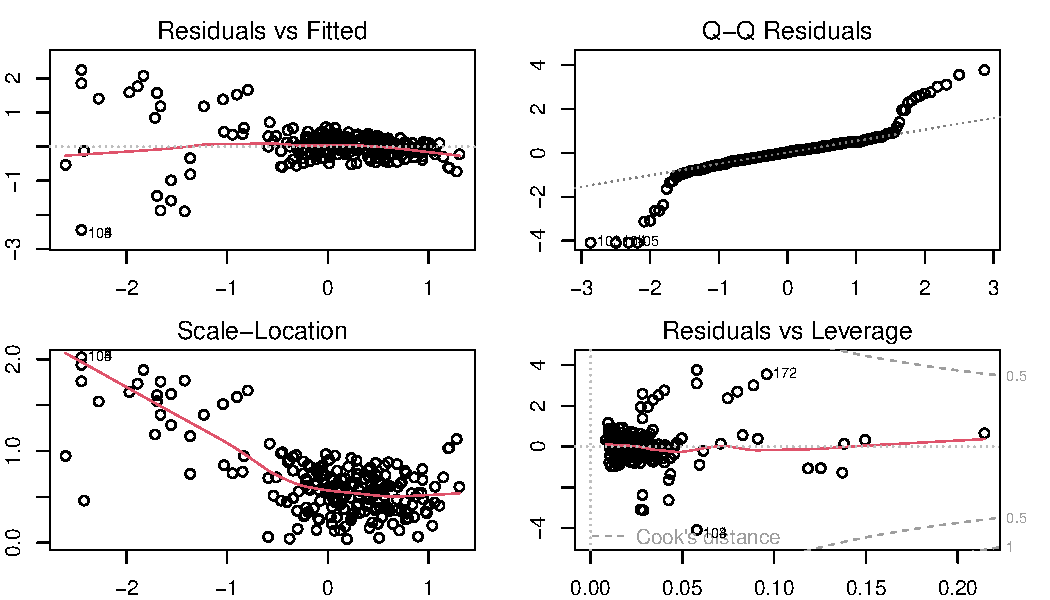
\includegraphics{Statistical_Learning_Final_Report_files/figure-latex/backward_elimination_log_2-1} \end{center}

\begin{Shaded}
\begin{Highlighting}[]
\FunctionTok{kable}\NormalTok{(}\FunctionTok{data.frame}\NormalTok{(}\AttributeTok{VIF =} \FunctionTok{vif}\NormalTok{(mod\_log\_tr\_backward\_2)),}
      \AttributeTok{caption =} \StringTok{"VIF values for the log transformed data with backward }
\StringTok{      elimination and manual removal of variables"}\NormalTok{)}
\end{Highlighting}
\end{Shaded}

\begin{longtable}[]{@{}lr@{}}
\caption{VIF values for the log transformed data with backward
elimination and manual removal of variables}\tabularnewline
\toprule\noalign{}
& VIF \\
\midrule\noalign{}
\endfirsthead
\toprule\noalign{}
& VIF \\
\midrule\noalign{}
\endhead
\bottomrule\noalign{}
\endlastfoot
Trans\_Fat & 1.491986 \\
Total\_Carbohydrates & 2.649737 \\
Protein & 10.478245 \\
Vitamin\_A & 8.772514 \\
Vitamin\_C & 1.241962 \\
Iron & 1.304571 \\
\end{longtable}

The VIF values are now below \(10\), indicating that multicollinearity
has been reduced in the model. The R-squared value is decreased but it
is still good.

\textbf{Model Diagnostics:} Non-normal residuals suggest that some
assumptions of linear regression might be violated. Specifically, the
assumption of normality of the residuals is not met, this can affect the
validity of hypothesis tests on the coefficients and predictions.

\begin{Shaded}
\begin{Highlighting}[]
\FunctionTok{shapiro.test}\NormalTok{((}\FunctionTok{residuals}\NormalTok{(mod\_log\_tr\_backward\_2)))}
\end{Highlighting}
\end{Shaded}

\begin{verbatim}
## 
##  Shapiro-Wilk normality test
## 
## data:  (residuals(mod_log_tr_backward_2))
## W = 0.82171, p-value = 5.816e-16
\end{verbatim}

Given the p-value is significantly smaller than \(0.05\), we reject the
null hypothesis. This indicates that the residuals of the model
\texttt{mod\_log\_tr\_backward\_2} do not follow a normal distribution.
In this case, W is quite a bit lower than \(1\), suggesting the
residuals deviate from normality. Sol Robust Methods: Use robust
regression methods that do not assume normality of errors.

We have tried other trasformation like min-max scaling and robust
scaling but not satisfactory due to VIF still to high. Regularization:
Using regularization methods such as ridge regression or lasso
regression penalizes the coefficients of variables, helping to reduce
multicollinearity.

\subsection{Lasso Regression}\label{lasso-regression}

We use the \texttt{glmnet} package to fit a lasso regression model.
Lasso regression, a type of linear regression that employs L1
regularization, penalizes the model's coefficients. This approach helps
prevent overfitting and identifies the most significant features in the
data.

First, we standardize the data and then fit the lasso regression model
using the \texttt{cv.glmnet} function. Cross-validation is employed to
select the optimal lambda value for the model. The lambda value that
minimizes the mean squared error (MSE) is chosen as the optimal value,
which is then used to fit the final lasso regression model.

Lasso regression tends to shrink the coefficients of less important
variables towards zero, effectively performing variable selection. By
eliminating irrelevant variables, it reduces the number of predictors
and, consequently, multicollinearity. Lasso regression often produces
sparse solutions by driving many coefficients to exactly zero. This
reduction in variables decreases multicollinearity among predictors,
resulting in lower Variance Inflation Factor (VIF) values. The automatic
feature selection inherent in lasso regression removes redundant
variables and reduces multicollinearity in the model.

\begin{Shaded}
\begin{Highlighting}[]
\NormalTok{std\_data }\OtherTok{\textless{}{-}} \FunctionTok{as.data.frame}\NormalTok{(}\FunctionTok{scale}\NormalTok{(data\_num)) }\CommentTok{\# Standardize the data}
\NormalTok{mod\_lasso }\OtherTok{\textless{}{-}} \FunctionTok{cv.glmnet}\NormalTok{(}\AttributeTok{x =} \FunctionTok{as.matrix}\NormalTok{(std\_data[, }\SpecialCharTok{{-}}\DecValTok{1}\NormalTok{]),}
                       \AttributeTok{y =}\NormalTok{ std\_data}\SpecialCharTok{$}\NormalTok{Calories, }\AttributeTok{alpha =} \DecValTok{1}\NormalTok{, }\AttributeTok{standardize =} \ConstantTok{FALSE}\NormalTok{)}
\FunctionTok{par}\NormalTok{(}\AttributeTok{mfrow =} \FunctionTok{c}\NormalTok{(}\DecValTok{1}\NormalTok{, }\DecValTok{1}\NormalTok{))}
\FunctionTok{plot}\NormalTok{(mod\_lasso, }\AttributeTok{xvar =} \StringTok{"lambda"}\NormalTok{, }\AttributeTok{label =} \ConstantTok{TRUE}\NormalTok{)}
\end{Highlighting}
\end{Shaded}

\begin{center}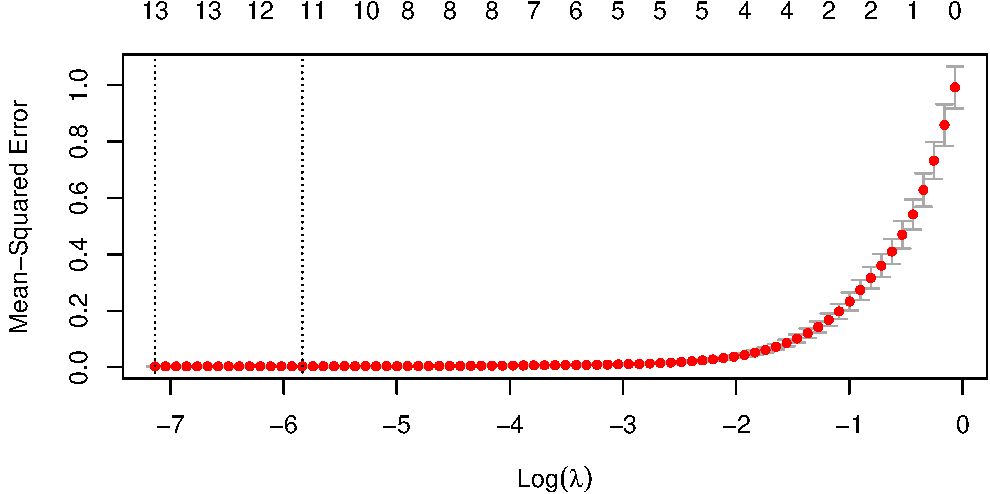
\includegraphics{Statistical_Learning_Final_Report_files/figure-latex/lasso_regression-1} \end{center}

By setting some coefficients to zero (such as
\texttt{"Saturated\_Fat"}), lasso regression aids in feature selection,
thereby reducing the model's complexity. The remaining non-zero
coefficients indicate the variables that significantly contribute to
predicting calories. The signs and magnitudes of these coefficients
illustrate the direction and strength of their relationships with the
target variable (\texttt{"calories"}). For example, a one-unit increase
in sodium, holding all other variables constant, is associated with a
decrease of approximately \(0.021\) calories.

The \texttt{cv.glmnet} function performs cross-validation to determine
the lambda value that minimizes the prediction error, identified as
\texttt{lambda.min}. In our case, we found that the optimal lambda value
is equal to \(1\).

To further evaluate the model's performance, metrics such as R-squared
and Mean Squared Error (MSE) should be considered. These metrics help in
understanding how well the model explains the variance in the data and
the average error of the predictions, respectively. Additionally, the
lambda value that minimizes the MSE is selected as the optimal lambda
value.

\subsection{Ridge Regression}\label{ridge-regression}

We also tried ridge regression to reduce multicollinearity. Like lasso
regression, ridge regression is a regularization technique that
introduces a penalty term to shrink coefficients towards zero without
eliminating them entirely, meaning that all variables can remain in the
model. Unlike lasso, which can zero out some coefficients and thus
perform variable selection, ridge regression retains all variables,
making it suitable for reducing multicollinearity without excluding any
variables. Lasso may be preferred when selecting a subset of the most
relevant variables is desired.

We use the \texttt{glmnet} package to fit a ridge regression model.
Ridge regression, a type of linear regression, uses L2 regularization to
penalize the coefficients of the model. This approach helps prevent
overfitting and reduces the impact of collinearity in the data.

The ridge regression model is fit using the \texttt{cv.glmnet()}
function, which incorporates cross-validation to determine the optimal
lambda value. Similar to lasso, the best lambda value, which minimizes
the error, was found to be equal to 1. The interpretation of the
coefficients is the same as in lasso regression.

\begin{Shaded}
\begin{Highlighting}[]
\NormalTok{mod\_ridge }\OtherTok{\textless{}{-}} \FunctionTok{cv.glmnet}\NormalTok{(}\AttributeTok{x =} \FunctionTok{as.matrix}\NormalTok{(std\_data[, }\SpecialCharTok{{-}}\DecValTok{1}\NormalTok{]),}
                       \AttributeTok{y =}\NormalTok{ std\_data}\SpecialCharTok{$}\NormalTok{Calories, }\AttributeTok{alpha =} \DecValTok{0}\NormalTok{, }\AttributeTok{standardize =} \ConstantTok{FALSE}\NormalTok{)}
\FunctionTok{plot}\NormalTok{(mod\_ridge, }\AttributeTok{xvar =} \StringTok{"lambda"}\NormalTok{, }\AttributeTok{label =} \ConstantTok{TRUE}\NormalTok{)}
\end{Highlighting}
\end{Shaded}

\begin{center}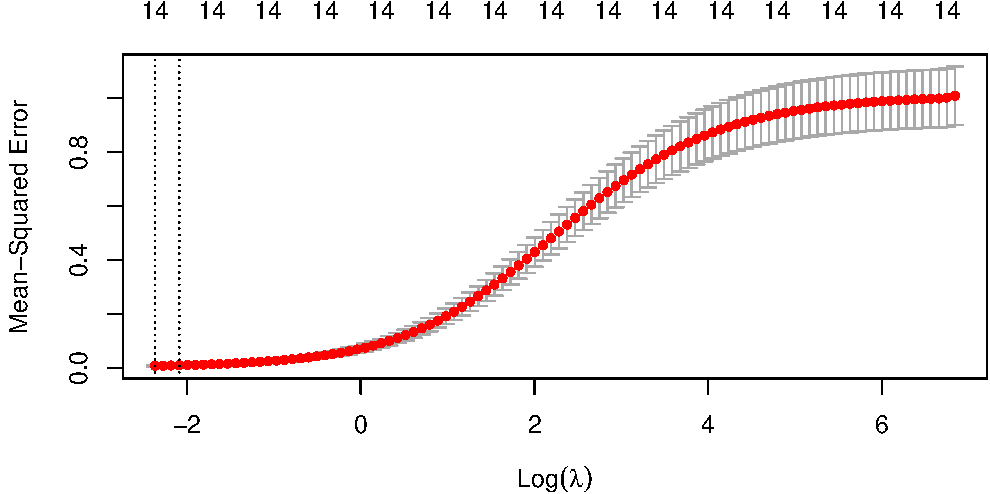
\includegraphics{Statistical_Learning_Final_Report_files/figure-latex/ridge_regression-1} \end{center}

\subsection{Model Comparison}\label{model-comparison}

We compare the linear regression, lasso regression, and ridge regression
models to select the best model for predicting the amount of calories
based on the amount of the other variables. We evaluate the models using
the R-squared value, and the Mean Squared Error (MSE) for each model.

The R-squared value is a measure of how well the model fits the data, it
ranges from \(0\) to \(1\), with higher values indicating a better fit

\begin{Shaded}
\begin{Highlighting}[]
\NormalTok{lasso\_pred }\OtherTok{\textless{}{-}} \FunctionTok{predict}\NormalTok{(mod\_lasso, }\AttributeTok{s =} \StringTok{"lambda.min"}\NormalTok{, }\AttributeTok{newx =} \FunctionTok{as.matrix}\NormalTok{(std\_data[, }\SpecialCharTok{{-}}\DecValTok{1}\NormalTok{]))}
\NormalTok{lasso\_r\_squared }\OtherTok{\textless{}{-}} \FunctionTok{cor}\NormalTok{(lasso\_pred, std\_data}\SpecialCharTok{$}\NormalTok{Calories)}\SpecialCharTok{\^{}}\DecValTok{2}
\NormalTok{ridge\_pred }\OtherTok{\textless{}{-}} \FunctionTok{predict}\NormalTok{(mod\_ridge, }\AttributeTok{s =} \StringTok{"lambda.min"}\NormalTok{,  }\AttributeTok{newx =} \FunctionTok{as.matrix}\NormalTok{(std\_data[, }\SpecialCharTok{{-}}\DecValTok{1}\NormalTok{]))}
\NormalTok{ridge\_r\_squared }\OtherTok{\textless{}{-}} \FunctionTok{cor}\NormalTok{(ridge\_pred, std\_data}\SpecialCharTok{$}\NormalTok{Calories)}\SpecialCharTok{\^{}}\DecValTok{2}
\FunctionTok{kable}\NormalTok{(}\FunctionTok{data.frame}\NormalTok{(}\AttributeTok{Model =} \FunctionTok{c}\NormalTok{(}\StringTok{"Linear Regression"}\NormalTok{, }\StringTok{"Lasso Regression"}\NormalTok{,}\StringTok{"Ridge Regression"}\NormalTok{),}
                 \AttributeTok{R\_squared =} \FunctionTok{c}\NormalTok{(}\FunctionTok{summary}\NormalTok{(lm\_model)}\SpecialCharTok{$}\NormalTok{r.squared,}
\NormalTok{                               lasso\_r\_squared, ridge\_r\_squared)), }
      \AttributeTok{caption =} \StringTok{"R{-}squared values for the models"}\NormalTok{)}
\end{Highlighting}
\end{Shaded}

\begin{longtable}[]{@{}lr@{}}
\caption{R-squared values for the models}\tabularnewline
\toprule\noalign{}
Model & R\_squared \\
\midrule\noalign{}
\endfirsthead
\toprule\noalign{}
Model & R\_squared \\
\midrule\noalign{}
\endhead
\bottomrule\noalign{}
\endlastfoot
Linear Regression & 0.9976608 \\
Lasso Regression & 0.9975756 \\
Ridge Regression & 0.9941815 \\
\end{longtable}

Comment on Lasso: The R-squared value of approximately \(0.998\)
indicates that the Lasso regression model explains about \(99.76\)\% of
the variance in the Calories variable. This suggests a very strong fit,
as the model is capturing almost all the variability in the target
variable.

Comment on Ridge: Similar to LASSO, very high

\subsection{Model Evaluation}\label{model-evaluation}

We evaluate the performance of the linear regression, lasso regression,
and ridge regression models using the mean squared error (MSE). The MSE
is a measure of the average squared difference between the predicted and
actual values. Lower values of the MSE indicate better performance of
the model.

\begin{Shaded}
\begin{Highlighting}[]
\NormalTok{linear\_pred }\OtherTok{\textless{}{-}} \FunctionTok{predict}\NormalTok{(lm\_model, }\AttributeTok{newdata =}\NormalTok{ data\_num)}
\NormalTok{linear\_mse }\OtherTok{\textless{}{-}} \FunctionTok{mean}\NormalTok{((linear\_pred }\SpecialCharTok{{-}}\NormalTok{ data\_num}\SpecialCharTok{$}\NormalTok{Calories)}\SpecialCharTok{\^{}}\DecValTok{2}\NormalTok{)}
\NormalTok{lasso\_mse }\OtherTok{\textless{}{-}} \FunctionTok{mean}\NormalTok{((lasso\_pred }\SpecialCharTok{{-}}\NormalTok{ std\_data}\SpecialCharTok{$}\NormalTok{Calories)}\SpecialCharTok{\^{}}\DecValTok{2}\NormalTok{)}
\NormalTok{ridge\_mse }\OtherTok{\textless{}{-}} \FunctionTok{mean}\NormalTok{((ridge\_pred }\SpecialCharTok{{-}}\NormalTok{ std\_data}\SpecialCharTok{$}\NormalTok{Calories)}\SpecialCharTok{\^{}}\DecValTok{2}\NormalTok{)}
\FunctionTok{kable}\NormalTok{(}\FunctionTok{data.frame}\NormalTok{(}\AttributeTok{Model =} \FunctionTok{c}\NormalTok{(}\StringTok{"Linear Regression"}\NormalTok{, }\StringTok{"Lasso Regression"}\NormalTok{, }\StringTok{"Ridge Regression"}\NormalTok{),}
                 \AttributeTok{MSE =} \FunctionTok{c}\NormalTok{(linear\_mse, lasso\_mse, ridge\_mse)), }
      \AttributeTok{caption =} \StringTok{"MSE values for the models"}\NormalTok{)}
\end{Highlighting}
\end{Shaded}

\begin{longtable}[]{@{}lr@{}}
\caption{MSE values for the models}\tabularnewline
\toprule\noalign{}
Model & MSE \\
\midrule\noalign{}
\endfirsthead
\toprule\noalign{}
Model & MSE \\
\midrule\noalign{}
\endhead
\bottomrule\noalign{}
\endlastfoot
Linear Regression & 24.6481166 \\
Lasso Regression & 0.0024158 \\
Ridge Regression & 0.0066477 \\
\end{longtable}

We choose the model with the highest R-squared value and the lowest MSE
as the best model for predicting the amount of calories based on the
amount of the other variables. The best model is the lasso because it
has the lowest value for R\^{}2 and MSE and it is the most robust model.

Comment on Lasso: The Mean Squared Error (MSE) of approximately
\(0.0024\) indicates a very low average squared difference between the
observed actual outcomes and the outcomes predicted by the model. This
suggests that the model's predictions are very close to the actual
values, indicating high accuracy. The optimal lambda value is used to
fit the final lasso regression model

?????????????????????? we want to check is Lasso regression has
effectvily reduced the multicollinearity, so we calculated the VIF on
predictors resulted by fitted Lasso, by looking at coefficients and
correlation matrix

Calcola i VIF TENERE????????????????????????? The variables
\texttt{"Total\_Fat"}, \texttt{"Trans\_Fat"}, \texttt{"Sodium"},
\texttt{"Total\_Carbohydrates"}, \texttt{"Cholesterol"},
\texttt{"Dietary\_Fibre"}, \texttt{"Sugars"}, \texttt{"Protein"},
\texttt{"Vitamin\_A"}, \texttt{"Vitamin\_C"}, \texttt{"Calcium"},
\texttt{"Iron"}, and \texttt{"Caffeine"} have coefficients of
significant magnitudes, suggesting that these variables are important
for predicting calories. Despite the regularization of the Lasso model,
some variables have coefficients of significant magnitudes, which could
suggest that these variables are not strongly correlated with each
other, thus reducing the impact of multicollinearity. Overall, the
absence of coefficients with very large magnitudes and the presence of
coefficients close to zero for some variables suggest that the Lasso
model may have helped mitigate multicollinearity and select only the
most important variables for predicting calories.

\subsection{Cross Validation}\label{cross-validation}

Cross validation is a technique used to evaluate the performance of a
model. It involves splitting the data into training and testing sets,
fitting the model using the training set, and evaluating the model using
the testing set. We decided to split the data with \(80\)\% of examples
for training and \(20\)\% for testing.

\begin{Shaded}
\begin{Highlighting}[]
\FunctionTok{set.seed}\NormalTok{(}\DecValTok{123}\NormalTok{)}
\NormalTok{train\_index }\OtherTok{\textless{}{-}} \FunctionTok{sample}\NormalTok{(}\DecValTok{1}\SpecialCharTok{:}\FunctionTok{nrow}\NormalTok{(std\_data), }\FloatTok{0.8} \SpecialCharTok{*} \FunctionTok{nrow}\NormalTok{(std\_data))}
\NormalTok{train\_data }\OtherTok{\textless{}{-}}\NormalTok{ std\_data[train\_index, ]}
\NormalTok{test\_data }\OtherTok{\textless{}{-}}\NormalTok{ std\_data[}\SpecialCharTok{{-}}\NormalTok{train\_index, ]}
\NormalTok{mod\_lasso\_train }\OtherTok{\textless{}{-}} \FunctionTok{cv.glmnet}\NormalTok{(}\AttributeTok{x =} \FunctionTok{as.matrix}\NormalTok{(train\_data[, }\SpecialCharTok{{-}}\DecValTok{1}\NormalTok{]), }\AttributeTok{y =}\NormalTok{ train\_data}\SpecialCharTok{$}\NormalTok{Calories,}
                             \AttributeTok{alpha =} \DecValTok{1}\NormalTok{, }\AttributeTok{standardize =} \ConstantTok{FALSE}\NormalTok{)}
\end{Highlighting}
\end{Shaded}

We evaluate the model using the testing set. We make predictions using
the testing set and calculate the mean squared error and the root mean
squared error to assess the model's accuracy.

\begin{Shaded}
\begin{Highlighting}[]
\NormalTok{lasso\_pred\_test }\OtherTok{\textless{}{-}} \FunctionTok{predict}\NormalTok{(mod\_lasso\_train, }\AttributeTok{s =} \StringTok{"lambda.min"}\NormalTok{,}
                           \AttributeTok{newx =} \FunctionTok{as.matrix}\NormalTok{(test\_data[, }\SpecialCharTok{{-}}\DecValTok{1}\NormalTok{]))}
\NormalTok{lasso\_r\_squared\_test }\OtherTok{\textless{}{-}} \FunctionTok{cor}\NormalTok{(lasso\_pred\_test, test\_data}\SpecialCharTok{$}\NormalTok{Calories)}\SpecialCharTok{\^{}}\DecValTok{2}
\NormalTok{lasso\_mse\_test }\OtherTok{\textless{}{-}} \FunctionTok{mean}\NormalTok{((lasso\_pred\_test }\SpecialCharTok{{-}}\NormalTok{ test\_data}\SpecialCharTok{$}\NormalTok{Calories)}\SpecialCharTok{\^{}}\DecValTok{2}\NormalTok{)}
\end{Highlighting}
\end{Shaded}

The R-squared value and MSE are used to evaluate the performance of the
model on the test data. Overall, the high R-squared value and low MSE on
the test data suggest that the lasso regression model has learned
effectively from the training data and generalizes well to unseen
examples.

\begin{Shaded}
\begin{Highlighting}[]
\NormalTok{accuracy\_lm }\OtherTok{\textless{}{-}} \DecValTok{1} \SpecialCharTok{{-}}\NormalTok{ (lasso\_mse\_test }\SpecialCharTok{/} \FunctionTok{var}\NormalTok{(test\_data}\SpecialCharTok{$}\NormalTok{Calories))}
\FunctionTok{par}\NormalTok{(}\AttributeTok{mfrow =} \FunctionTok{c}\NormalTok{(}\DecValTok{1}\NormalTok{, }\DecValTok{1}\NormalTok{), }\AttributeTok{mar =} \FunctionTok{c}\NormalTok{(}\DecValTok{4}\NormalTok{, }\DecValTok{4}\NormalTok{, }\DecValTok{2}\NormalTok{, }\DecValTok{2}\NormalTok{))}
\FunctionTok{plot}\NormalTok{(test\_data}\SpecialCharTok{$}\NormalTok{Calories, lasso\_pred\_test, }\AttributeTok{xlab =} \StringTok{"Actual Calories"}\NormalTok{, }\AttributeTok{col =} \StringTok{"\#99cfad"}\NormalTok{,}
     \AttributeTok{ylab =} \StringTok{"Predicted Calories"}\NormalTok{, }\AttributeTok{main =} \StringTok{"Predicted vs Actual Calories"}\NormalTok{, }\AttributeTok{pch =} \DecValTok{19}\NormalTok{)}
\FunctionTok{abline}\NormalTok{(}\DecValTok{0}\NormalTok{, }\DecValTok{1}\NormalTok{, }\AttributeTok{col =} \StringTok{"\#258894"}\NormalTok{, }\AttributeTok{lwd =} \DecValTok{2}\NormalTok{)}
\end{Highlighting}
\end{Shaded}

\begin{center}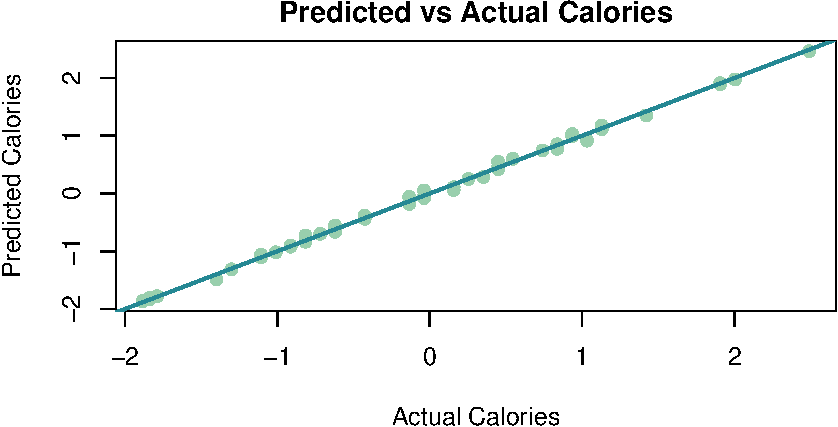
\includegraphics{Statistical_Learning_Final_Report_files/figure-latex/accuracy_lm-1} \end{center}

\begin{Shaded}
\begin{Highlighting}[]
\FunctionTok{kable}\NormalTok{(}\FunctionTok{data.frame}\NormalTok{(}\AttributeTok{Accuracy =}\NormalTok{ accuracy\_lm, }\AttributeTok{MSE =}\NormalTok{ lasso\_mse\_test, }
                 \AttributeTok{R\_squared =}\NormalTok{ lasso\_r\_squared\_test),}
      \AttributeTok{caption =} \StringTok{"Model evaluation metrics on the test data"}\NormalTok{)}
\end{Highlighting}
\end{Shaded}

\begin{longtable}[]{@{}lrrr@{}}
\caption{Model evaluation metrics on the test data}\tabularnewline
\toprule\noalign{}
& Accuracy & MSE & R\_squared \\
\midrule\noalign{}
\endfirsthead
\toprule\noalign{}
& Accuracy & MSE & R\_squared \\
\midrule\noalign{}
\endhead
\bottomrule\noalign{}
\endlastfoot
lambda.min & 0.9979473 & 0.0026283 & 0.9979454 \\
\end{longtable}

\begin{Shaded}
\begin{Highlighting}[]
\NormalTok{lasso\_mse\_test}
\end{Highlighting}
\end{Shaded}

\begin{verbatim}
## [1] 0.002628338
\end{verbatim}

As we can see from \emph{Table X} the R-squared value is \(0.997\),
indicating that the model explains \(99\)\% of the variance in the data
and the MSE is \(0.002628338\), indicating that the model has a low
error rate. The accuracy of the model is \(0.9979473\), indicating that
the model is able to predict the amount of calories with high accuracy.
The plot shows the predicted values against the actual values on the
test data, as we can see the points are close to the diagonal line,
indicating that the model is making accurate predictions.

\subsection{Logistic Regression}\label{logistic-regression}

Logistic regression is a statistical model used to predict the outcome
of a binary categorical dependent variable based on one or more
independent variables. Since logistic regression is tipycally used for
classification task and our variable Calories ,that we want to predict
is continous random variable, we have to traspose the problem into a
classification one by making the variable binary. In order to do that we
classify foods into two categories: ``low calorie'' and ``high
calories'' defining a threshold to distinguish between the two classes.

let's take a look into the structure of the variable using numeric
dataset only

We've tried with normal data, standardize data, and log trasformation
since again it helps to reduce multicollinearity and we find out that
the best is with log trasformed data looking at the summary and the plot
of the variable, we notice that calories follow a semi-gaussian
distribution both Median and mean are reasonable approach to use, since
they are close to each other. However we choose median as treshold is
less sensitive to outliers and skewness in the data. It ensures that
half the data points are classified as \texttt{"low\ calories"} and the
other half as \texttt{"high\ calories"}, providing balanced classes.

\begin{Shaded}
\begin{Highlighting}[]
\NormalTok{y }\OtherTok{\textless{}{-}}\NormalTok{ std\_data\_log\_df}\SpecialCharTok{$}\NormalTok{Calories}
\NormalTok{calories\_median }\OtherTok{\textless{}{-}} \FunctionTok{median}\NormalTok{(y)}
\CommentTok{\# Create a new binary target variable based on the median}
\NormalTok{std\_data\_log\_df}\SpecialCharTok{$}\NormalTok{Calorie\_Class }\OtherTok{\textless{}{-}} \FunctionTok{ifelse}\NormalTok{(std\_data\_log\_df}\SpecialCharTok{$}\NormalTok{Calories }\SpecialCharTok{\textgreater{}}\NormalTok{ calories\_median, }\DecValTok{1}\NormalTok{, }\DecValTok{0}\NormalTok{)}
\FunctionTok{table}\NormalTok{(std\_data\_log\_df}\SpecialCharTok{$}\NormalTok{Calorie\_Class)}
\end{Highlighting}
\end{Shaded}

\begin{verbatim}
## 
##   0   1 
## 121 121
\end{verbatim}

\begin{Shaded}
\begin{Highlighting}[]
\CommentTok{\# Creates a new binary variable (Calorie\_Class) where 1 indicates high calorie }
\CommentTok{\# (above median) and 0 indicates low calorie (below or equal to median).}

\CommentTok{\# Fit a logistic regression model on the complete dataset obatines with }
\CommentTok{\# log tasformation and by removing first column }
\NormalTok{logistic\_model }\OtherTok{\textless{}{-}} \FunctionTok{glm}\NormalTok{(Calorie\_Class }\SpecialCharTok{\textasciitilde{}}\NormalTok{ ., }\AttributeTok{data =}\NormalTok{ std\_data\_log\_df[,}\SpecialCharTok{{-}}\DecValTok{1}\NormalTok{], }\AttributeTok{family =}\NormalTok{ binomial)}
\FunctionTok{kable}\NormalTok{(}\FunctionTok{data.frame}\NormalTok{(}\AttributeTok{AIC =} \FunctionTok{AIC}\NormalTok{(logistic\_model), }\AttributeTok{BIC =} \FunctionTok{BIC}\NormalTok{(logistic\_model), }
                 \AttributeTok{Residual\_deviance =}\NormalTok{ logistic\_model}\SpecialCharTok{$}\NormalTok{deviance,}
                 \AttributeTok{Null\_deviance =}\NormalTok{ logistic\_model}\SpecialCharTok{$}\NormalTok{null.deviance,}
                 \AttributeTok{R\_squared =} \DecValTok{1} \SpecialCharTok{{-}}\NormalTok{ logistic\_model}\SpecialCharTok{$}\NormalTok{deviance }\SpecialCharTok{/}\NormalTok{ logistic\_model}\SpecialCharTok{$}\NormalTok{null.deviance),}
      \AttributeTok{caption =} \StringTok{"Model evaluation metrics for the logistic regression model"}\NormalTok{)}
\end{Highlighting}
\end{Shaded}

\begin{longtable}[]{@{}rrrrr@{}}
\caption{Model evaluation metrics for the logistic regression
model}\tabularnewline
\toprule\noalign{}
AIC & BIC & Residual\_deviance & Null\_deviance & R\_squared \\
\midrule\noalign{}
\endfirsthead
\toprule\noalign{}
AIC & BIC & Residual\_deviance & Null\_deviance & R\_squared \\
\midrule\noalign{}
\endhead
\bottomrule\noalign{}
\endlastfoot
69.42364 & 121.7577 & 39.42364 & 335.4832 & 0.882487 \\
\end{longtable}

\begin{Shaded}
\begin{Highlighting}[]
\FunctionTok{par}\NormalTok{(}\AttributeTok{mfrow =} \FunctionTok{c}\NormalTok{(}\DecValTok{2}\NormalTok{, }\DecValTok{2}\NormalTok{), }\AttributeTok{mar =} \FunctionTok{c}\NormalTok{(}\DecValTok{2}\NormalTok{, }\DecValTok{2}\NormalTok{, }\DecValTok{2}\NormalTok{, }\DecValTok{2}\NormalTok{))}
\FunctionTok{plot}\NormalTok{(logistic\_model)}
\end{Highlighting}
\end{Shaded}

\begin{center}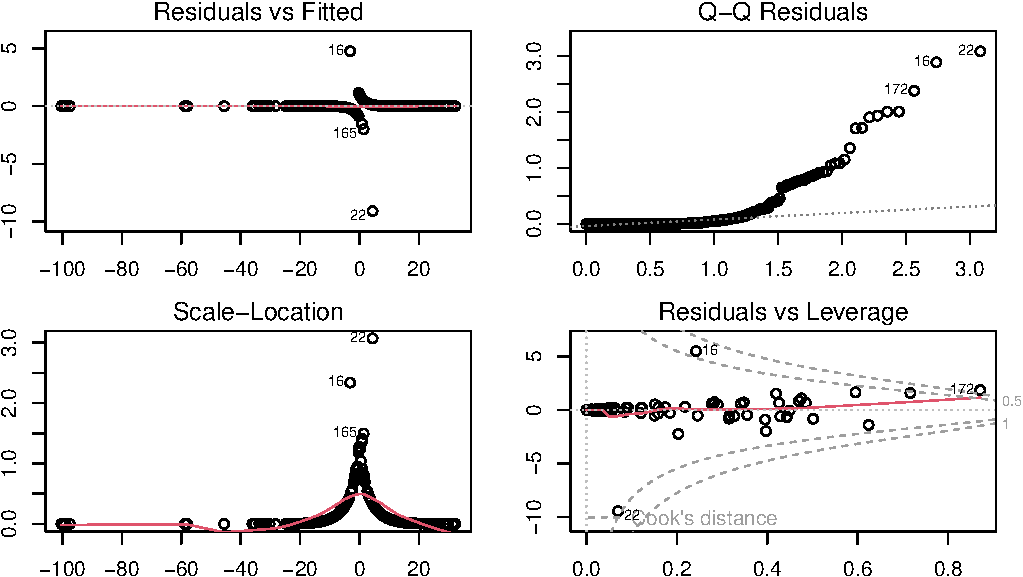
\includegraphics{Statistical_Learning_Final_Report_files/figure-latex/logistic_regression-1} \end{center}

The statistically significant coefficient of the model are
\texttt{"Cholesterol"} at the 0.01 level and \texttt{"Total\_Fat"} at
the 0.05 level. The residual deviance is much smaller than the null
deviance, indicating that the model with predictors explains more
variability than the null model. The AIC is 69.424, suggesting that the
model has reasonable fit. Number of Fisher Scoring Iterations: Indicates
the number of iterations performed by the Fisher scoring algorithm
during model fitting. In this case, it took 11 iterations.

Now we use the model to make predictions on the data and evaluate its
performance using the confusion matrix, accuracy, precision, recall, and
F1-score.

\begin{Shaded}
\begin{Highlighting}[]
\NormalTok{conf\_matrix }\OtherTok{\textless{}{-}} \FunctionTok{table}\NormalTok{(}\AttributeTok{Predicted =}\NormalTok{ predicted\_classes, }\AttributeTok{Actual =}\NormalTok{ new\_test\_data}\SpecialCharTok{$}\NormalTok{Calorie\_Class)}
\FunctionTok{kable}\NormalTok{(conf\_matrix, }\AttributeTok{caption =} \StringTok{"Confusion matrix for the logistic regression model"}\NormalTok{)}
\end{Highlighting}
\end{Shaded}

\begin{longtable}[]{@{}lrr@{}}
\caption{Confusion matrix for the logistic regression
model}\tabularnewline
\toprule\noalign{}
& 0 & 1 \\
\midrule\noalign{}
\endfirsthead
\toprule\noalign{}
& 0 & 1 \\
\midrule\noalign{}
\endhead
\bottomrule\noalign{}
\endlastfoot
0 & 22 & 2 \\
1 & 2 & 23 \\
\end{longtable}

\begin{Shaded}
\begin{Highlighting}[]
\NormalTok{accuracy }\OtherTok{\textless{}{-}}\NormalTok{ (conf\_matrix[}\DecValTok{1}\NormalTok{, }\DecValTok{1}\NormalTok{] }\SpecialCharTok{+}\NormalTok{ conf\_matrix[}\DecValTok{2}\NormalTok{, }\DecValTok{2}\NormalTok{]) }\SpecialCharTok{/} \FunctionTok{sum}\NormalTok{(conf\_matrix)}
\NormalTok{precision }\OtherTok{\textless{}{-}}\NormalTok{ conf\_matrix[}\DecValTok{2}\NormalTok{, }\DecValTok{2}\NormalTok{] }\SpecialCharTok{/} \FunctionTok{sum}\NormalTok{(conf\_matrix[, }\DecValTok{2}\NormalTok{])}
\NormalTok{recall }\OtherTok{\textless{}{-}}\NormalTok{ conf\_matrix[}\DecValTok{2}\NormalTok{, }\DecValTok{2}\NormalTok{] }\SpecialCharTok{/} \FunctionTok{sum}\NormalTok{(conf\_matrix[}\DecValTok{2}\NormalTok{, ])}
\NormalTok{f1\_score }\OtherTok{\textless{}{-}} \DecValTok{2} \SpecialCharTok{*}\NormalTok{ (precision }\SpecialCharTok{*}\NormalTok{ recall) }\SpecialCharTok{/}\NormalTok{ (precision }\SpecialCharTok{+}\NormalTok{ recall)}
\FunctionTok{kable}\NormalTok{(}\FunctionTok{data.frame}\NormalTok{(}\AttributeTok{Accuracy =}\NormalTok{ accuracy, }\AttributeTok{Precision =}\NormalTok{ precision, }\AttributeTok{Recall =}\NormalTok{ recall,}
                 \AttributeTok{F1\_Score =}\NormalTok{ f1\_score), }\AttributeTok{caption =} \StringTok{"Model evaluation metrics"}\NormalTok{)}
\end{Highlighting}
\end{Shaded}

\begin{longtable}[]{@{}rrrr@{}}
\caption{Model evaluation metrics}\tabularnewline
\toprule\noalign{}
Accuracy & Precision & Recall & F1\_Score \\
\midrule\noalign{}
\endfirsthead
\toprule\noalign{}
Accuracy & Precision & Recall & F1\_Score \\
\midrule\noalign{}
\endhead
\bottomrule\noalign{}
\endlastfoot
0.9183673 & 0.92 & 0.92 & 0.92 \\
\end{longtable}

The model's accuracy of approximately 91.8\% indicates it is performing
well overall in classifying the calorie content correctly. Generalize
well on the test set

\begin{Shaded}
\begin{Highlighting}[]
\FunctionTok{par}\NormalTok{(}\AttributeTok{mfrow =} \FunctionTok{c}\NormalTok{(}\DecValTok{2}\NormalTok{,}\DecValTok{2}\NormalTok{), }\AttributeTok{mar =} \FunctionTok{c}\NormalTok{(}\DecValTok{2}\NormalTok{, }\DecValTok{2}\NormalTok{, }\DecValTok{2}\NormalTok{, }\DecValTok{2}\NormalTok{))}
\FunctionTok{plot}\NormalTok{(logistic\_model\_train)}
\end{Highlighting}
\end{Shaded}

\begin{center}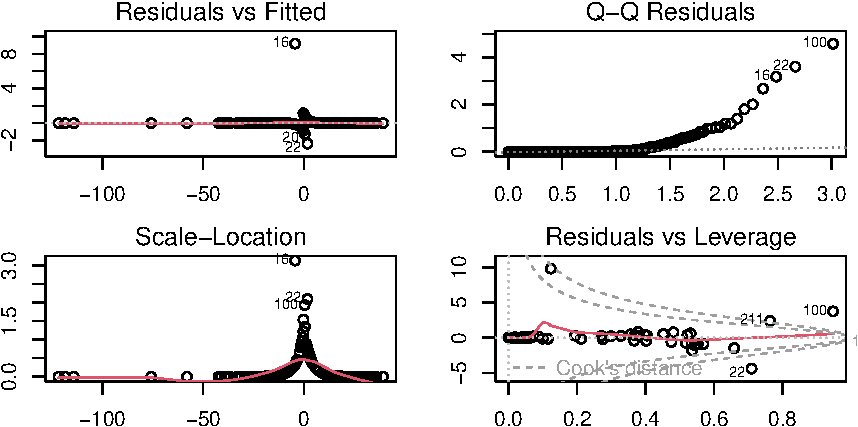
\includegraphics{Statistical_Learning_Final_Report_files/figure-latex/logistic_regression_evaluation_2-1} \end{center}

\textbf{Residuals vs Fitted:}

This plot shows the Pearson residuals against the fitted values.
Ideally, there should be no clear pattern, indicating that the model is
well-fitted. However, the presence of data points at extreme values (far
from 0) suggests potential issues with model fit or outliers.

\textbf{Normal Q-Q Plot:}

The Q-Q plot compares the standardized deviance residuals to a
theoretical normal distribution. Significant deviations from the
straight line suggest that the residuals are not normally distributed,
which can indicate potential problems with the model. In this case, the
data points deviate from the line, particularly at the higher quantiles,
indicating that the residuals are not perfectly normally distributed.

\textbf{Scale-Location Plot (Spread-Location Plot):} This plot shows the
square root of the standardized residuals against the fitted values. The
red line helps to identify trends. Ideally, the points should be
randomly scattered without a clear pattern. Here, we see some clustering
and trends at extreme fitted values, suggesting heteroscedasticity or
non-constant variance.

\textbf{Residuals vs Leverage:} This plot shows standardized residuals
against leverage, highlighting influential data points. The dashed lines
represent Cook's distance. Points outside these lines indicate
influential observations that have a significant impact on the model. In
this plot, several points, especially at higher leverage values, fall
outside the dashed lines, indicating they are influential.

\textbf{Interpretation}

\textbf{Potential Issues with Model Fit:} The presence of extreme
residuals in the Residuals vs Fitted and Scale-Location plots suggests
that the model might not fit well across all observations. This can be
due to outliers or the model not capturing the underlying data structure
adequately.

\textbf{Non-Normal Residuals:} The Q-Q plot indicates that the residuals
are not perfectly normally distributed, which is expected in logistic
regression but still worth noting.

\textbf{Influential Points:} The Residuals vs Leverage plot shows
several influential points, suggesting that some observations have a
disproportionate impact on the model. These points should be
investigated further to understand their nature and whether they are
legitimate data points or outliers.

\textbf{Next Steps}

\textbf{Investigate Influential Points:} Check the data points
identified as influential in the Residuals vs Leverage plot to
understand why they have high leverage and residuals.

\textbf{Consider Model Refinement:} If certain variables consistently
show poor performance, it might be necessary to transform them, add
interaction terms, or consider alternative modeling techniques.

\textbf{Check for Multicollinearity:} Ensure that multicollinearity is
not affecting the model by calculating Variance Inflation Factors (VIFs)
for the predictors.

\textbf{Evaluate Model with Additional Metrics:} Use additional
performance metrics such as ROC AUC, Precision-Recall curves, and
confusion matrix to evaluate the model's predictive performance
comprehensively.

\end{document}
